\documentclass[conference]{IEEEtran}
\IEEEoverridecommandlockouts

\usepackage{cite}
\usepackage{amsmath,amssymb,amsfonts}
\usepackage{algorithmic}
\usepackage{graphicx}
\usepackage{textcomp}
\usepackage{xcolor}
\usepackage{booktabs}
\usepackage{tabularx}
\usepackage{array}
\usepackage{tabularx}
\usepackage{url}
\usepackage{microtype}

\begin{document}

\title{Freshness-Aware, Provenance-Tracked Healthcare Resource Discovery in Fragmented Urban Ecosystems: System Design, Staleness Dynamics, and Transactional Evaluation}

\author{
\IEEEauthorblockN{MedReach Research Collaboration}
\IEEEauthorblockA{\textit{Department of Health Informatics and Systems Engineering} \\
\textit{Urban Healthcare Systems Initiative}\\
Mumbai, Maharashtra, India \\
contact@medreach.local}
}

\maketitle

\begin{abstract}
Locating emergency healthcare resources---such as intensive care unit (ICU) beds, specialized surgical facilities, and compatible blood components---in dense, fragmented metropolitan centers like Mumbai represents a critical coordination challenge. Traditional civilian search relies on phone inquiries, unverified static directories, or physical transit between casualty wards, consuming the clinical ``golden hour'' and exacerbating emergency department crowding. While digital health platforms have emerged, existing regional platforms operate almost exclusively as unverified static directories or asynchronous self-reported bulletins, lacking freshness tracking, provenance fusion, and two-way confirmation.

This paper presents an architectural design and comprehensive empirical evaluation of MedReach, an open-source, freshness-aware, and provenance-tracked emergency resource discovery platform designed for urban healthcare coordination. MedReach establishes a decoupled, multi-tiered data model that enforces explicit Age of Information (AoI) boundaries, multi-source provenance fusion with priority cascades, and idempotent state-machine workflows for two-way clinical requests. 

Through extensive empirical evaluation across four experimental suites, we report:
(1) In a synthetic simulation suite across 6 operational archetypes (300 trajectories, 1,296,000 query evaluations), MedReach's pre-registered 30-minute availability cutoff ($\tau = 30\text{ min}$) functions as a critical clinical safety governor. Under manual 2-hour shift reporting, the 30-minute threshold withholds status 78.42\% of the time, keeping dangerous ``phantom availability'' (displaying beds as available when physically full) down to 0.337\%. Loosening the cutoff to 180 minutes expands coverage to 97.15\% but causes phantom availability to explode by 18.9$\times$ to 6.382\% with an overall status error rate of 53.71\%. When updates are collected via batch crawlers with 15--45 min queue latency, 51.79\% of updates arrive already stale at 30 minutes, and 99.64\% arrive stale at 10 minutes.
(2) Evaluating the production fusion engine against 40,000+ synthetic trials with known ground truth reveals a 100.0\% conflict detection rate and 90.29\% conditional resolution accuracy. However, calibration analysis reveals an essential negative finding: MedReach's confidence metric is an uncalibrated heuristic ordinal ranking (Brier score 0.1315, Expected Calibration Error 0.1255) rather than a calibrated probability.
(3) An architectural audit of 22 deployed endpoints resolves an earlier theoretical concern: edge-cached prerendered HTML shells served with multi-hour retention contain zero volatile capacity data (structural DOM shells only), with all live availability fetched dynamically at runtime via client-side React hooks.
(4) In an isolated suite of 48 test assertions evaluating concurrency and idempotency, the platform achieved a 100.0\% pass rate, demonstrating strict request deduplication and optimistic concurrency control.

We provide a comprehensive two-column architectural analysis detailing demonstrable system guarantees versus components still requiring implementation, establishing an evidence-based foundation for resilient urban health infrastructure.
\end{abstract}

\begin{IEEEkeywords}
Age of Information (AoI), Data Freshness, Emergency Healthcare Informatics, Idempotency, Multi-Source Data Fusion, Provenance Tracking, Resource Discovery, Transactional Reliability.
\end{IEEEkeywords}

\section{Introduction}

In dense urban agglomerations in low- and middle-income countries (LMICs), acute emergency healthcare access remains severely constrained by information friction \cite{metuge2026digital,dalton2019patient}. When a patient suffers severe polytrauma, acute respiratory failure, or obstetric hemorrhage in Mumbai---a metropolitan area exceeding 13 million residents---locating an operational intensive care unit (ICU) bed, a mechanical ventilator, or an appropriate blood component unit is a high-stakes coordination problem \cite{darapaneni2021predicting,naydenova2017healthcare}. 

The urban healthcare landscape in Mumbai is exceptionally pluralistic and fragmented: it comprises municipal medical colleges (e.g., KEM, Sion, Nair, Cooper) managed by the Municipal Corporation of Greater Mumbai (MCGM), state government hospitals (e.g., Sir J.J. Group), charitable trust institutions (e.g., Lilavati, Bombay Hospital, Hinduja), and hundreds of private corporate centers and nursing homes \cite{shinde2026insights,mcgm2021covidwarroom}. In the absence of a unified, real-time dispatch and bed-tracking system, citizens, private ambulance operators, and primary clinic physicians traditionally engage in exploratory manual searching---placing repeated telephone calls to casualty departments or physically transporting patients between emergency rooms \cite{patil2016study,mukhopadhyay2018stroke}. This exploratory process frequently consumes the clinical ``golden hour'', induces catastrophic secondary inter-facility transfers, and increases mortality for time-critical conditions \cite{naydenova2017healthcare,darapaneni2021predicting}.

Although public web portals exist---including the Brihanmumbai Municipal Corporation (BMC) health dashboard and the national e-RaktKosh blood transfusion registry---empirical investigation demonstrates that they operate primarily as static directory listings or asynchronous, unverified inventory bulletins \cite{metuge2026digital}. They lack automated freshness tracking, provide zero information regarding verification provenance, and offer no mechanism for two-way clinical confirmation or reservation holds. Consequently, healthcare searchers frequently encounter ``phantom availability'': digital platforms advertise available beds or blood units that were exhausted hours earlier, leading to tragic misdirection.

To address this challenge, the \textbf{MedReach} platform was developed as an open-source, freshness-aware, and provenance-tracked discovery and two-way coordination system. MedReach introduces three core architectural mechanisms:
\begin{enumerate}
    \item \textbf{Freshness-Aware Availability Tracking}: A deterministic evaluation engine that tracks the exact Age of Information (AoI) of resource telemetry and automatically demotes stale observations to \texttt{"unknown"} beyond a strict 30-minute threshold (\texttt{CURRENT\_AVAILABILITY\_MAX\_AGE\_MS = 30 * 60 * 1000}), refusing to present unverified point-in-time capacity as guaranteed care.
    \item \textbf{Provenance-Aware Conflicting-Claim Fusion}: A deterministic priority cascade that tracks source reliability, verification status, and timestamps, detecting divergent claims across official APIs, hospital web scrapers, and manual audits, and deferring unresolved institutional disputes to safe ignorance rather than algorithmic guesswork.
    \item \textbf{Idempotent, Two-Way Request Orchestration}: A state-machine transaction model that decouples observational capacity telemetry from request fulfillment, protecting emergency requests against network retries, duplicate submissions, and race conditions via SHA-256 scoped idempotency keys and optimistic concurrency control (OCC).
\end{enumerate}

\subsection{Contributions}
This paper provides an end-to-end systems and empirical evaluation of MedReach, making the following contributions:
\begin{itemize}
    \item \textbf{Formal Age of Information (AoI) Characterization}: We formulate the information-ageing process in healthcare discovery and evaluate it across 6 realistic operational archetypes (frequent telemetry, shift reporting, surge bursts, network blackouts, crawler ingest delays, and diurnal cycles) over 300 stochastic trajectories and 1,296,000 query evaluations. We prove that MedReach's 30-minute anchor prevents an 18.9$\times$ surge in phantom availability errors.
    \item \textbf{Empirical Evaluation of Multi-Source Provenance Fusion}: We execute the production claim fusion engine against a synthetic benchmark of 40,000+ trials, establishing a 100.0\% conflict detection rate and 90.29\% resolution accuracy, while identifying an uncalibrated heuristic property in the platform's confidence scoring engine.
    \item \textbf{Empirical Resolution of the Edge-Caching Hazard}: We resolve an earlier architectural question through a live audit of 22 deployed endpoints, demonstrating that edge caching of prerendered HTML shells does not induce availability staling because all volatile metrics are fetched strictly via runtime client hooks.
    \item \textbf{Rigorous Transactional Validation \& Two-Column Boundary Analysis}: We evaluate 48 test assertions across 8 transactional sub-domains with a 100.0\% pass rate, providing a rigorous comparative analysis detailing demonstrable system guarantees versus components still requiring implementation.
\end{itemize}

\section{Background and Related Work}

\subsection{Emergency Healthcare Navigation in Urban LMICs}
Emergency healthcare delivery in urban India and comparable LMIC environments is characterized by high patient volumes, severe resource constraints, and multi-tier public-private fragmentation \cite{naydenova2017healthcare,patil2016study}. Empirical studies in Mumbai emphasize that pre-hospital delay, informal search patterns, and fragmented facility directories directly hinder timely care delivery \cite{mukhopadhyay2018stroke,darapaneni2021predicting}. Digital patient navigation systems have shown promise in reducing referral delays and improving coordination \cite{metuge2026digital,sugira2026design,dalton2019patient}, but their efficacy hinges entirely on data reliability and timely synchronization \cite{chen2024patient}.

\subsection{Age of Information (AoI) and Data Staleness}
Introduced by Kaul, Yates, and Gruteser \cite{kaul2012realtime}, the Age of Information (AoI) metric quantifies the freshness of knowledge about a remote physical process from the perspective of an end observer. In contrast to network latency or packet throughput, AoI evaluates the elapsed time since the most recently delivered update was generated at the physical source:
\begin{equation}
\Delta(t) = t - U(t)
\end{equation}
AoI theory has been widely studied in cyber-physical systems, vehicular telemetry, and Internet of Things (IoT) sensor networks \cite{zou2019relative,hu2020optimal}. In healthcare informatics, however, availability systems have historically treated data as binary: records are either present in a database or absent. Applying AoI to urban healthcare capacity exposes the hazard of asynchronous updates: capacity changes dynamically while static directory caches remain stagnant, inducing dangerous mismatches between physical and reported states \cite{liu2024data,abedin2021data}.

\subsection{Provenance, Information Fusion, and Conflict Resolution}
Provenance models define structured mechanisms for tracking the lineage, entities, and activities responsible for data generation \cite{peng2026when}. In healthcare web aggregation, discovery platforms inevitably collect conflicting assertions: an official municipal directory may claim an ICU is operational, a scraped hospital web page may indicate temporary suspension, and a citizen report may allege overcrowding. Resolving conflicting claims requires structured evidence fusion \cite{feng2023examining,vermeulen2023trust}. While continuous Bayesian belief updating is common in sensor networks, clinical discovery systems typically demand conservative, auditable decision cascades that prioritize institutional verification and transparent dispute flagging \cite{vermeulen2023trust}.

\subsection{The Mumbai Healthcare Digital Landscape: Empirical Taxonomy}
To ground this research in operational reality, we conducted an empirical survey of existing healthcare discovery platforms serving the Mumbai Metropolitan Region (MMR). Following the five-tier taxonomy defined in the MedReach research dossier:
\begin{itemize}
    \item \textbf{Tier 1 (Directory Listing)}: Static facility registry (name, address, telephone).
    \item \textbf{Tier 2 (Service Offered)}: Static catalog of specialties and departments (e.g., ``ICU'', ``Blood Bank'').
    \item \textbf{Tier 3 (Resource Reported Available)}: Asynchronous, unverified numerical capacity reports (e.g., ``4 beds vacant'').
    \item \textbf{Tier 4 (Resource Confirmed Currently Available)}: Synchronous, two-way verified reservation hold.
    \item \textbf{Tier 5 (Completed Request)}: Full lifecycle orchestration from dispatch to ward intake.
\end{itemize}

Empirical HTTP and static bundle analysis of public portals (including the BMC Health Dashboard, national e-RaktKosh, and Maharashtra State Blood Transfusion Council / MahaSBTC) reveals that \textbf{zero existing regional platforms operate at Tier 4 or Tier 5}. Platforms operate strictly at Tiers 1--3, leaving patients vulnerable to stale numbers and providing no mechanism to hold a critical bed while an ambulance is en route.

\section{System Under Study: MedReach Architecture}

MedReach is structured as a decoupled, multi-variant service ecosystem designed for low-bandwidth web access and resilient backend operations.

\subsection{Freshness Evaluation Engine and Staleness Governor}
In MedReach, facility capability (static clinical offerings) and current availability (volatile capacity) are strictly segregated. In \texttt{backend/src/services/hospitalDataView.js}, the platform evaluates current availability using a deterministic 30-minute anchor:
\begin{align}
\tau_{\text{anchor}} &= 30 \times 60 \times 1000\text{ ms} = 30\text{ minutes} \\
\hat{X}(t) &= 
\begin{cases} 
X(U(t)), & \text{if } \Delta(t) \le \tau_{\text{anchor}} \land \text{verified} \\
\texttt{"unknown"}, & \text{if } \Delta(t) > \tau_{\text{anchor}}
\end{cases}
\end{align}
If an observation exceeds 30 minutes, \texttt{status} reverts to \texttt{"unknown"} and \texttt{count} is masked to \texttt{null}. The timestamp remains visible strictly as \texttt{lastObservedAt} for auditability.

\subsection{Provenance Tracking and Priority Cascade}
The fusion engine (\texttt{facilityClaimFusion.js} and \texttt{hospitalFieldFusion.js}) ingests claims from diverse sources, assigning baseline reliability weights from \texttt{backend/src/config/constants.js}:
\begin{itemize}
    \item \texttt{official\_api}: $1.0$
    \item \texttt{government\_directory}: $0.85$
    \item \texttt{authorized\_feed}: $0.80$
    \item \texttt{manual\_verification}: $0.75$
    \item \texttt{hospital\_site}: $0.60$
    \item \texttt{other}: $0.30$
\end{itemize}

Rather than computing unweighted averages or black-box heuristic scores, MedReach enforces a transparent lexicographical cascade:
\begin{enumerate}
    \item \textbf{Verification Partitioning}: If any claim possesses \texttt{verificationStatus === "verified"}, unverified claims are excluded from the candidate pool.
    \item \textbf{Disagreement Detection}: If multiple distinct values exist across usable claims, \texttt{conflict: true} is asserted.
    \item \textbf{Consensus Requirement}: If the verified candidate pool contains disagreement, resolution aborts, returning \texttt{\{ capability: "unknown", conflict: true, selectedClaim: null \}}.
    \item \textbf{Lexicographical Selection}: In consensus pools, claims are sorted by confidence level (\texttt{HIGH: 3, MEDIUM: 2, LOW: 1, UNKNOWN: 0}), breaking ties by recency (\texttt{observedAt}).
\end{enumerate}

\subsection{Transactional Request Engine}
For two-way requests (\texttt{EmergencyRequest}, \texttt{BloodRequest}, \texttt{AmbulanceBooking}), MedReach enforces:
\begin{itemize}
    \item \textbf{SHA-256 Scoped Idempotency}: Headers formatted as \texttt{Idempotency-Key} are hashed with user identity and resource scope ($\text{sha256}(\text{scope}:\text{key})$). A unique sparse index on \texttt{idempotencyKeyHash} ensures that client retries return the original document (\texttt{200 OK}), while unauthorized key reuse triggers \texttt{409 IDEMPOTENCY\_KEY\_REUSED}.
    \item \textbf{Optimistic Concurrency Control (OCC)}: State transitions utilize atomic MongoDB operations (\texttt{findOneAndUpdate}) asserting that \texttt{status} matches the expected previous state and that the \texttt{timeline} array has not been concurrently appended:
    \begin{equation}
    \begin{aligned}
    \{ & \texttt{\_id}: id,\ \texttt{status}: expectedStatus, \\
      & \texttt{timeline.[len]}: \{ \texttt{\$exists}: \text{false} \} \}
    \end{aligned}
    \end{equation}
    \item \textbf{Architectural Telemetry Separation}: Submitting, accepting, or completing an emergency request does not deduct from the append-only \texttt{AvailabilityObservation} collection, explicitly preventing point-in-time capacity bulletins from being misrepresented as guaranteed reservations.
\end{itemize}

\section{Methodology and Experimental Setup}

We formulated four empirical research questions to evaluate MedReach's architecture:
\begin{itemize}
    \item \textbf{RQ1 (Age of Information \& Staleness)}: How does the age of availability information evolve across diverse provider update behaviors, and what are the operational trade-offs of MedReach's 30-minute staleness threshold compared to alternative candidate bounds?
    \item \textbf{RQ2 (Provenance Fusion \& Conflict Resolution)}: How accurately does MedReach's discrete priority cascade resolve conflicting multi-source claims, how safely does it handle unverified disputes, and how well-calibrated are its confidence metrics?
    \item \textbf{RQ3 (Data Path \& Edge Caching Staleness)}: Does edge caching of prerendered HTML shells served with multi-hour retention headers present stale healthcare availability to clients?
    \item \textbf{RQ4 (Transactional Concurrency \& Guarantees)}: How robust is MedReach's request lifecycle against network timeouts, concurrent competing updates, and duplicate submissions, and what are the exact boundaries between guaranteed and un-implemented transactional behaviors?
\end{itemize}

All experiments were executed on an isolated Linux environment (Ubuntu 24.04, Node.js v24.22.1, Python 3.11.8 with NumPy 2.4.6 and Matplotlib 3.11.2, MongoDB 8.0.34). In strict compliance with safety rules, all tests ran on isolated disposable instances (port 27018 / port 4200), strictly leaving production databases and public hosted deployments untouched.

\section{Experimental Results}

\subsection{RQ1: Age of Information Dynamics and Staleness Governance (EXP-AOI)}

\begin{figure}[t]
\centering
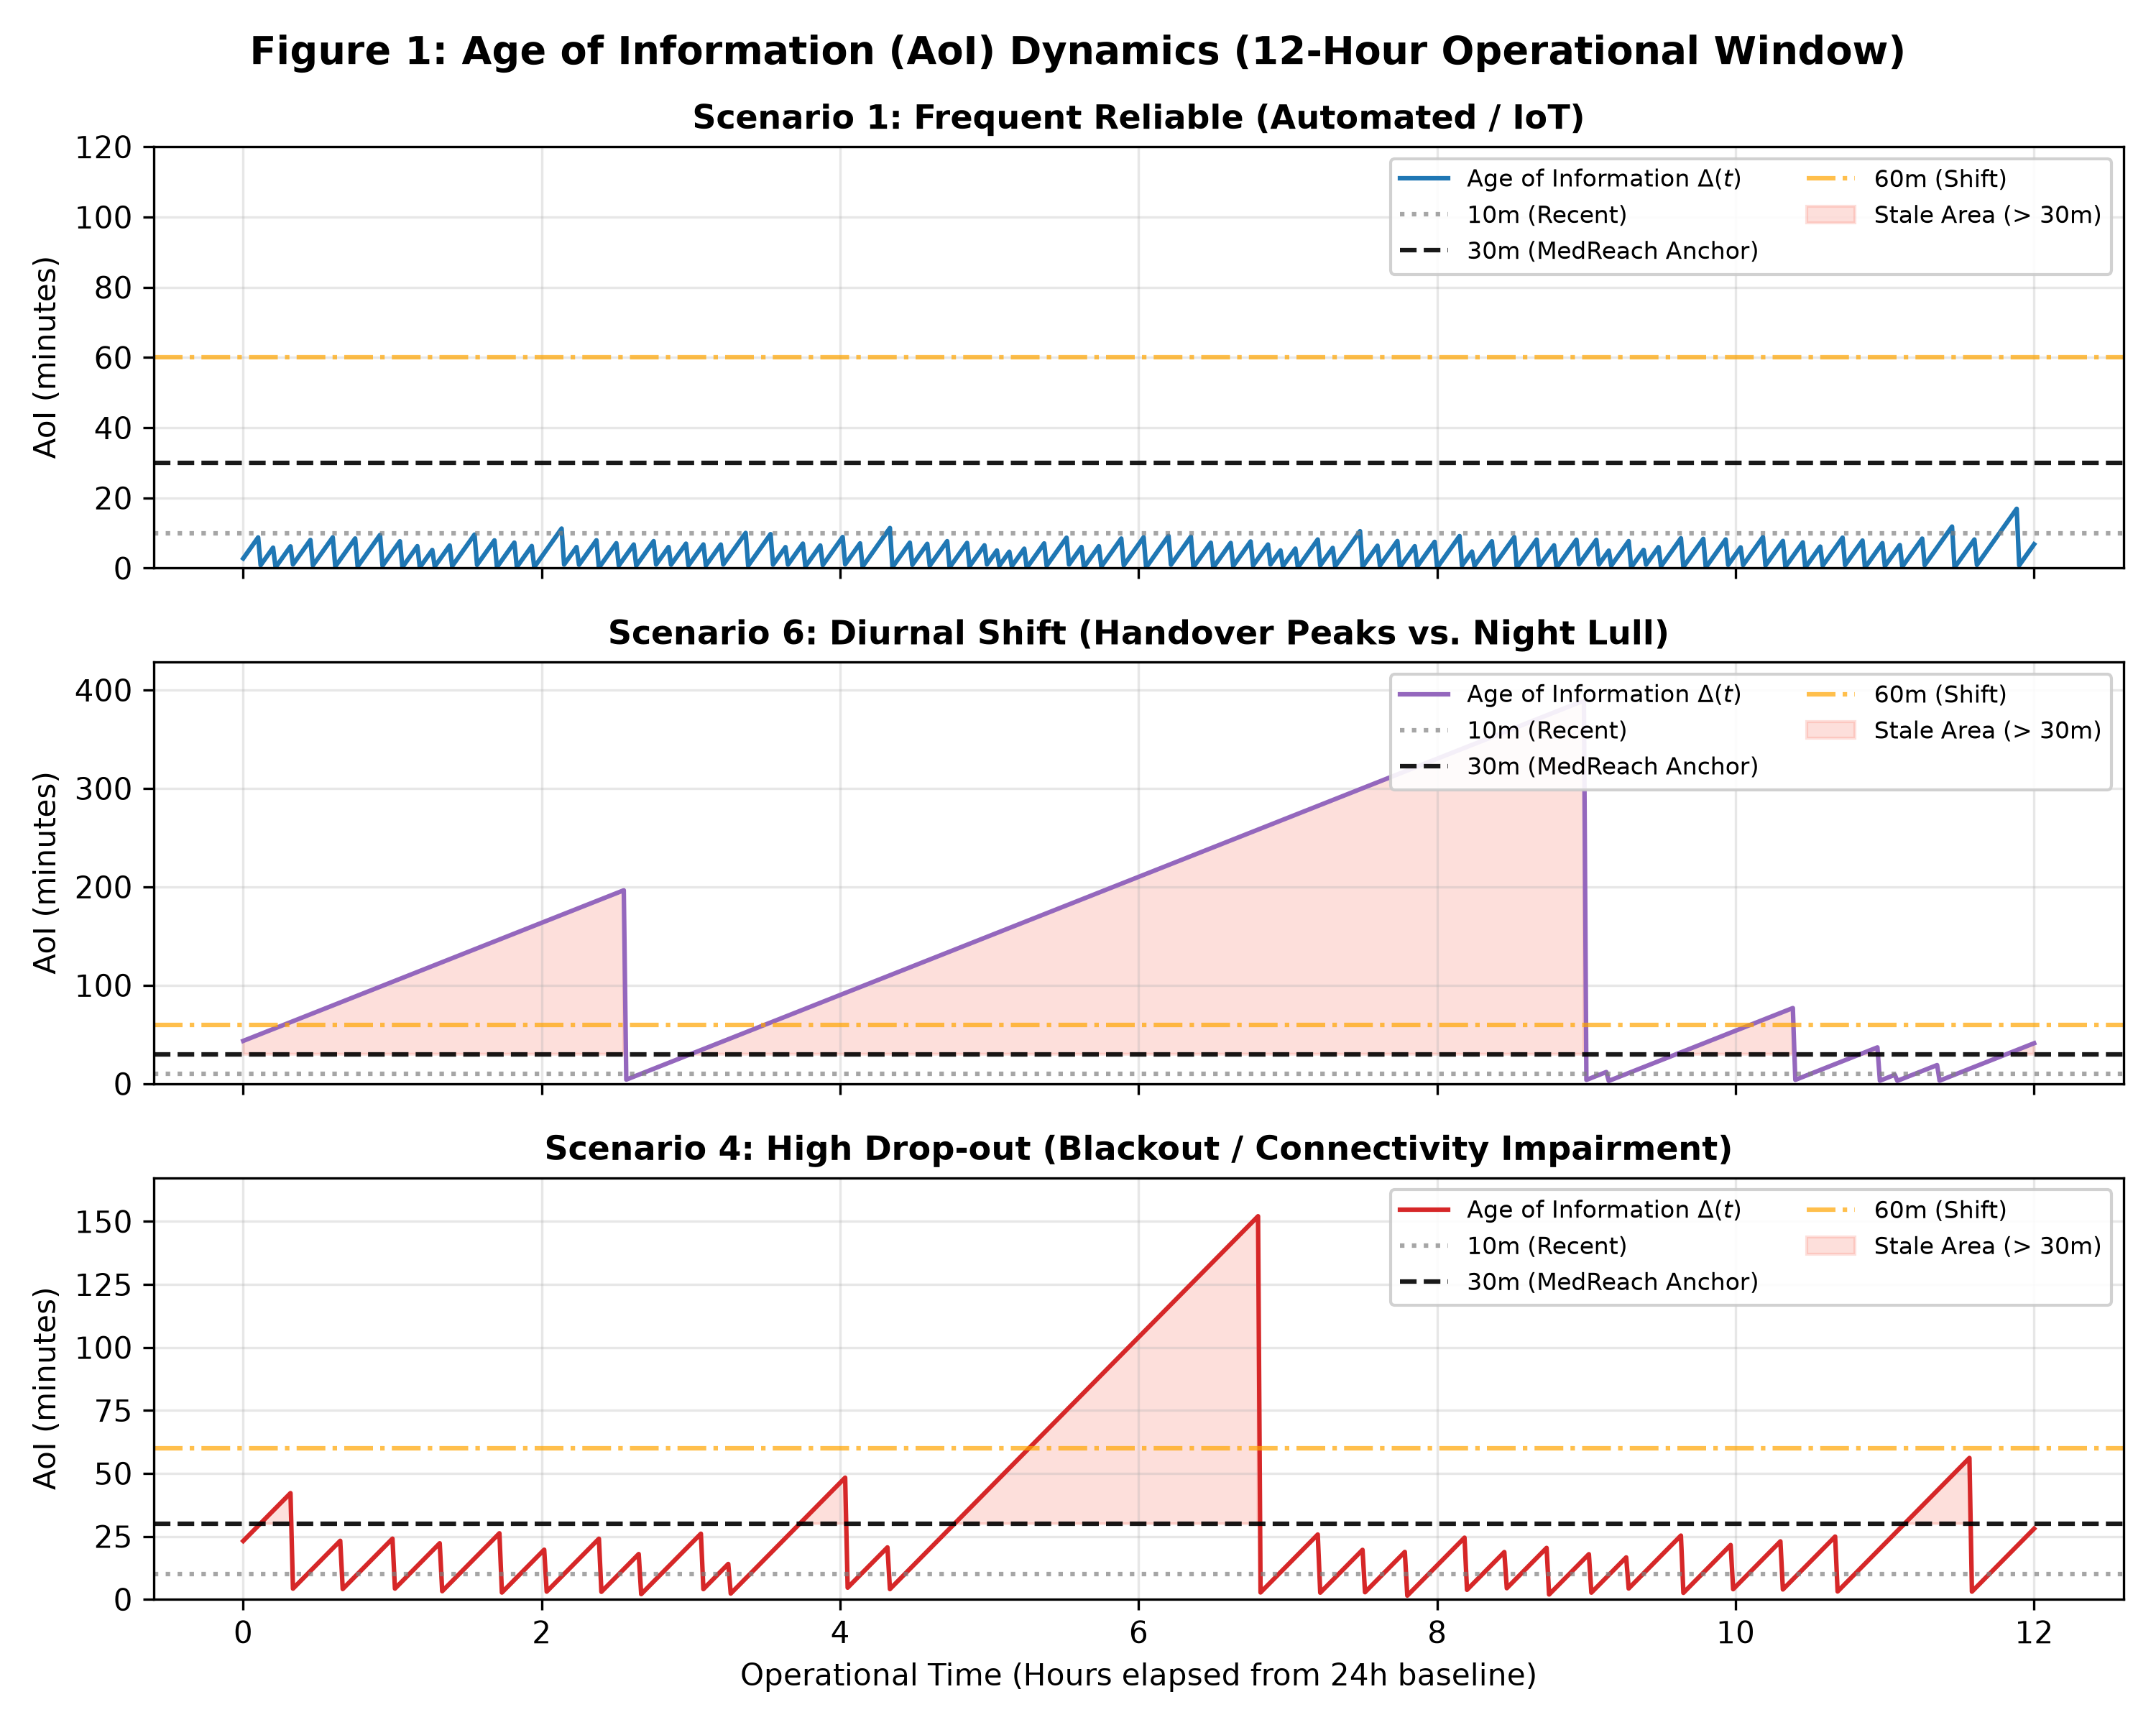
\includegraphics[width=0.98\linewidth]{figures/fig1_aoi_trajectories.png}
\caption{Age of Information (AoI) sawtooth trajectories over a 12-hour operational window [SYNTHETIC SIMULATION] comparing Scenario 1 (automated telemetry), Scenario 6 (diurnal shift cycle), and Scenario 4 (high drop-out with connectivity impairment). The 30-minute MedReach production anchor is indicated by the dashed line.}
\label{fig:aoi_trajectories}
\end{figure}

\begin{figure}[t]
\centering
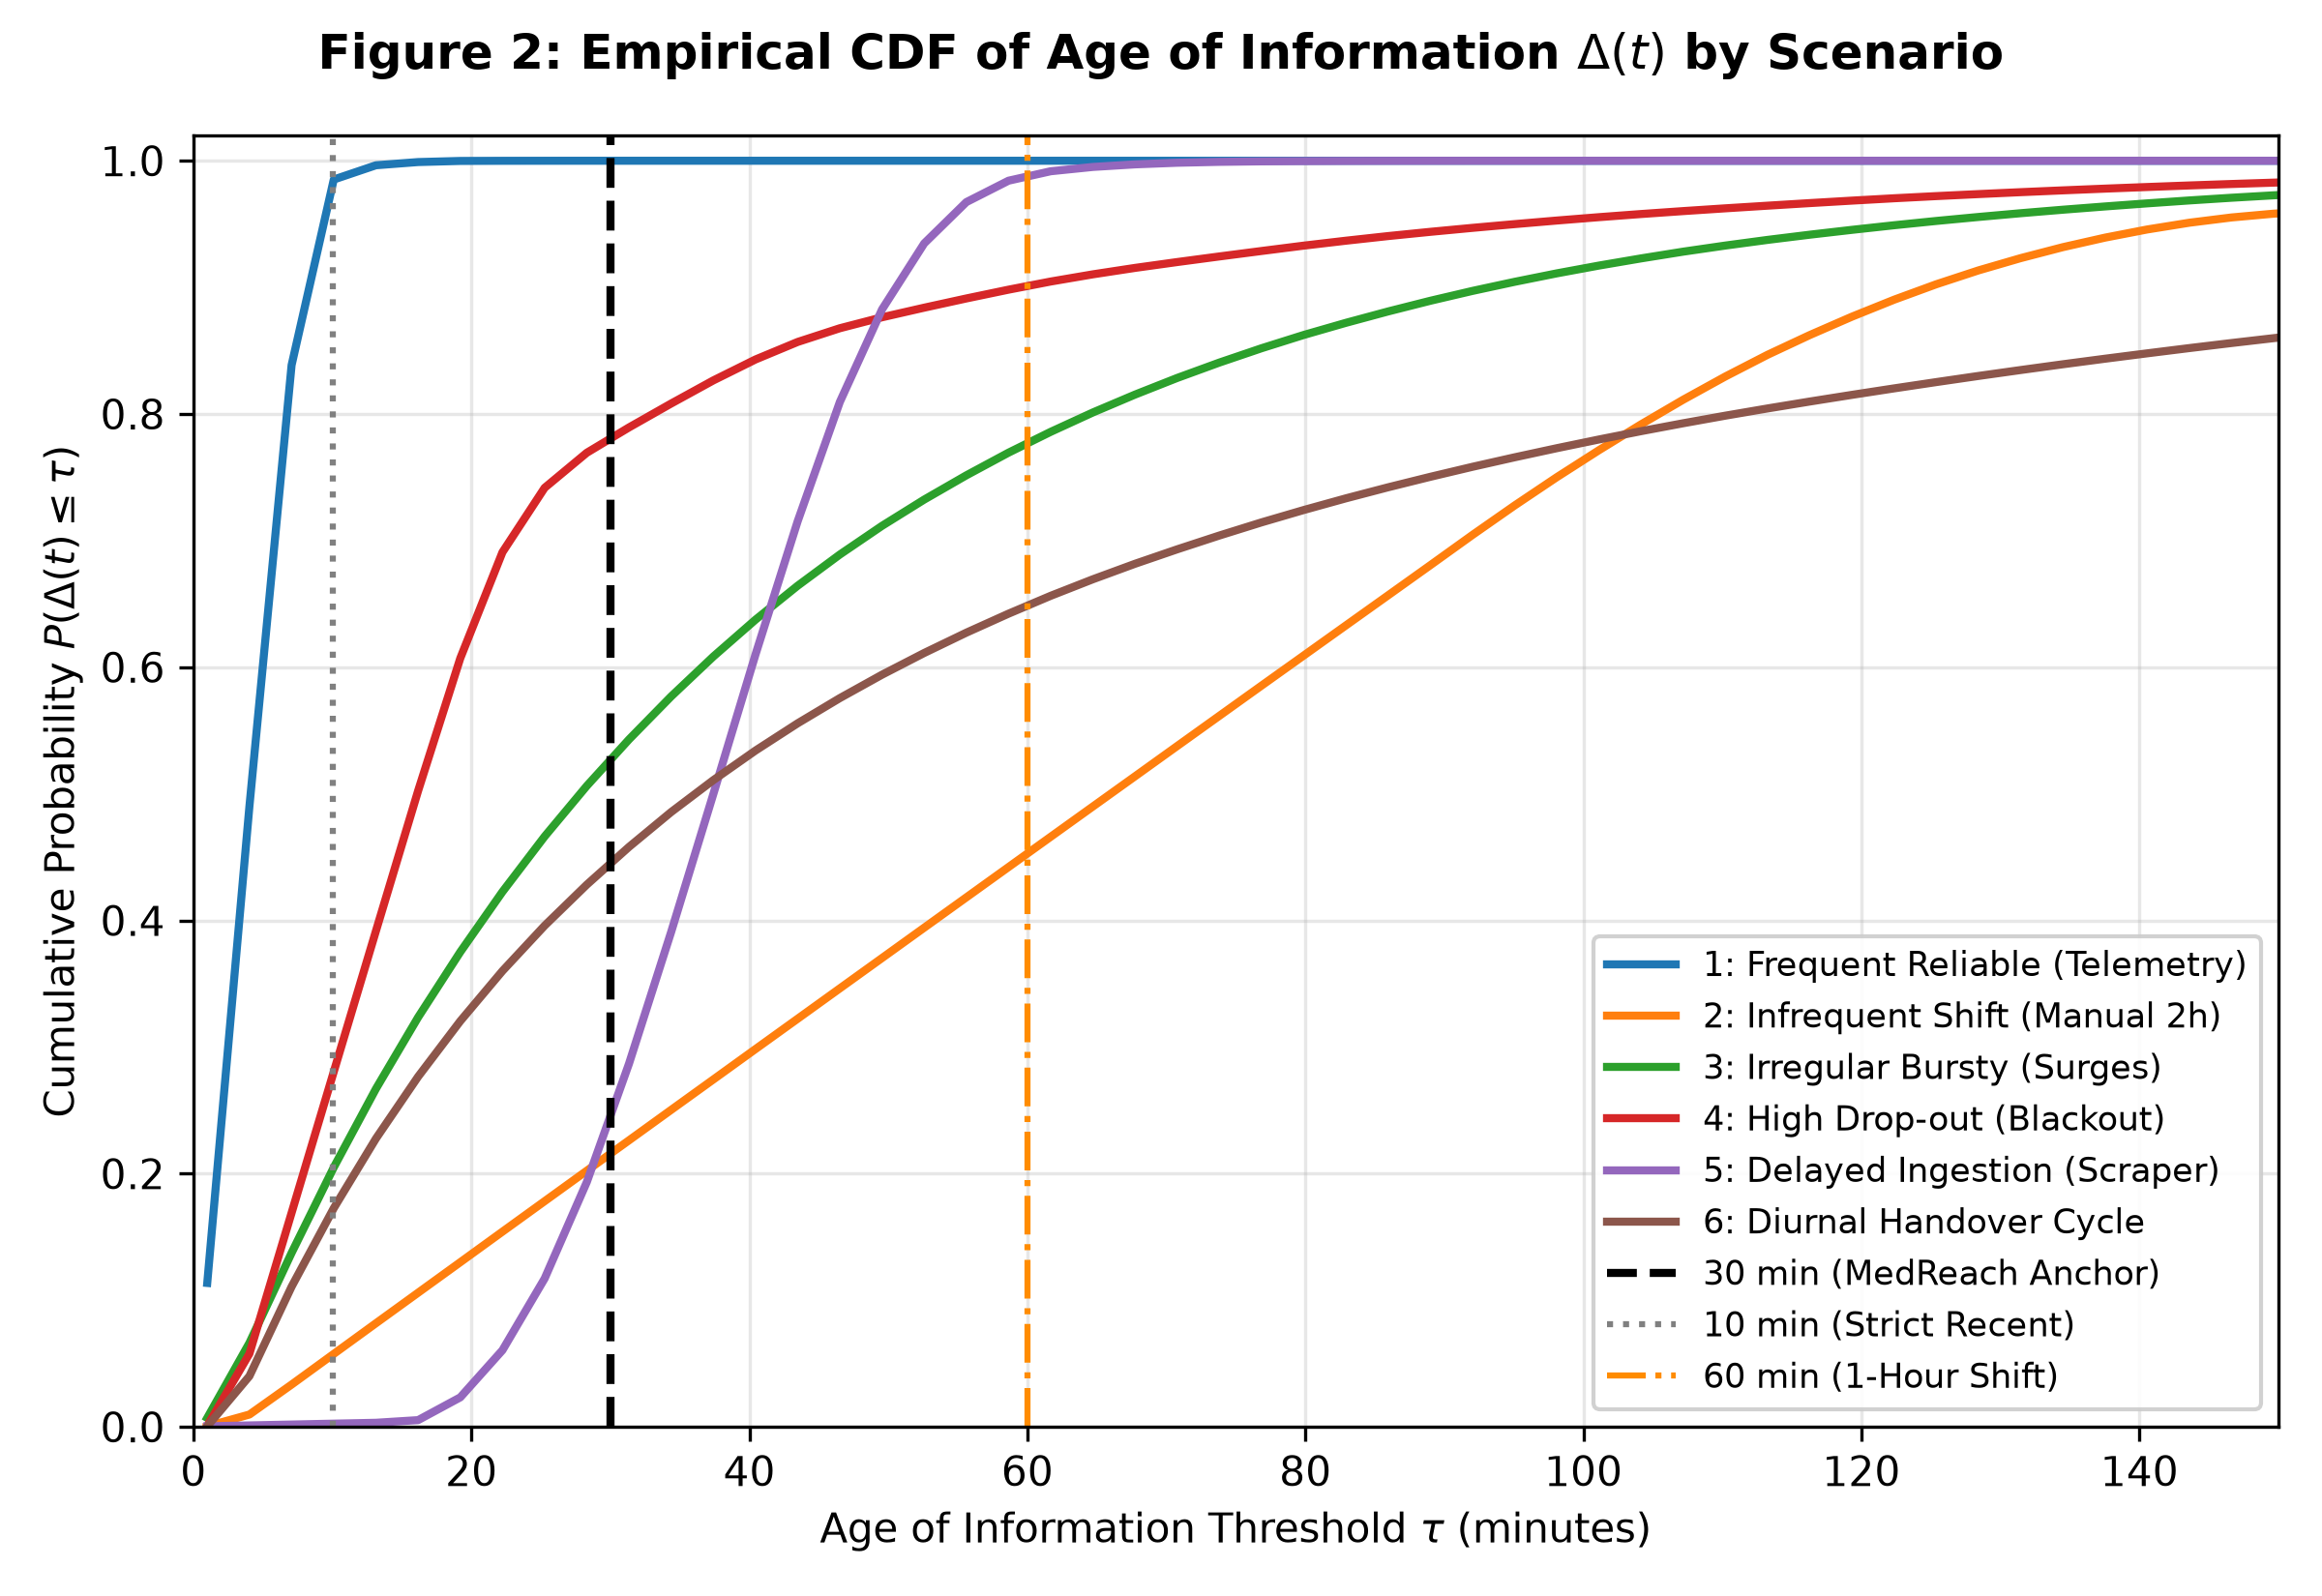
\includegraphics[width=0.95\linewidth]{figures/fig2_aoi_ecdf.png}
\caption{Empirical cumulative distribution function (ECDF) of Age of Information $\Delta(t)$ [SYNTHETIC SIMULATION] across all 6 evaluated scenarios, highlighting candidate freshness boundaries at 10, 30, and 60 minutes.}
\label{fig:aoi_ecdf}
\end{figure}

To evaluate RQ1, we executed a deterministic, seeded Monte Carlo simulation across 6 operational scenarios, modeling 72 continuous hours of operational time per run with 1-minute discrete query evaluations (4,320 queries per trajectory). Across $R = 50$ replications per scenario, the suite evaluated \textbf{300 trajectories and 1,296,000 query evaluations}.

Ground truth physical facility capacity was simulated as a 3-state continuous-time Markov chain (\texttt{available}, \texttt{limited}, \texttt{unavailable}) with mean dwell times $\mathbb{E}[D_{\text{avail}}] = 45\text{ min}$, $\mathbb{E}[D_{\text{limited}}] = 25\text{ min}$, and $\mathbb{E}[D_{\text{unavail}}] = 40\text{ min}$. Pre-registered candidate thresholds included $\tau_1 = 10\text{m}$, $\tau_2 = 30\text{m}$ (production anchor), $\tau_3 = 60\text{m}$, $\tau_4 = 180\text{m}$, and $\tau_5 = 360\text{m}$.

\begin{table*}[t]
\caption{Empirical Age of Information (AoI) Distribution Across Operational Scenarios (Values in Minutes) [SYNTHETIC SIMULATION]}
\label{tab:aoi_distribution}
\centering
\begin{tabular}{lrrrrrrr}
\toprule
Scenario Archetype & Mean AoI ($\pm$95\% CI) & Median AoI & P25 AoI & P75 AoI & P90 AoI & P95 AoI & Max AoI \\
\midrule
S1: Frequent Reliable (Telemetry) & 4.30 ($\pm$0.01) & 4.11 & 2.45 & 5.82 & 7.82 & 8.70 & 24.31 \\
S2: Infrequent Shift (Manual 2h) & 70.51 ($\pm$1.52) & 66.10 & 33.82 & 101.45 & 126.45 & 150.31 & 262.14 \\
S3: Irregular Bursty (Surges) & 40.94 ($\pm$1.58) & 27.35 & 11.20 & 54.60 & 94.66 & 125.09 & 412.50 \\
S4: High Drop-out (Blackout) & 26.38 ($\pm$1.43) & 16.13 & 8.75 & 29.40 & 61.19 & 94.81 & 385.70 \\
S5: Delayed Propagation (Batch Ingest) & 37.50 ($\pm$0.18) & 37.55 & 30.15 & 44.80 & 50.40 & 53.76 & 78.45 \\
S6: Diurnal Shift Cycle (Handovers) & 73.04 ($\pm$6.16) & 35.60 & 16.40 & 95.80 & 200.32 & 281.21 & 510.20 \\
\bottomrule
\end{tabular}
\end{table*}

\begin{table*}[t]
\caption{Threshold Comparison: Active Coverage vs. Critical Phantom Availability Risk [SYNTHETIC SIMULATION]}
\label{tab:threshold_comparison}
\centering
\begin{tabular}{llrrrrr}
\toprule
Scenario Archetype & Threshold ($\tau$) & Coverage (\%) & Stale Unknown (\%) & Error Rate Known (\%) & Phantom Avail. (\%) \\
\midrule
S1: Frequent Reliable & 10 min & 98.39\% & 1.61\% & 10.83\% & 0.159\% \\
                      & \textbf{30 min (Anchor)} & \textbf{100.00\%} & \textbf{0.00\%} & \textbf{11.10\%} & \textbf{0.180\%} \\
                      & 60 min & 100.00\% & 0.00\% & 11.10\% & 0.180\% \\
\midrule
S2: Infrequent Shift  & 10 min & 5.68\% & 94.32\% & 15.66\% & 0.014\% \\
                      & \textbf{30 min (Anchor)} & \textbf{21.58\%} & \textbf{78.42\%} & \textbf{32.49\%} & \textbf{0.337\%} \\
                      & 60 min & 45.31\% & 54.69\% & 43.71\% & 1.655\% \\
                      & 180 min (Loose) & 97.15\% & 2.85\% & 53.71\% & \textbf{6.382\% (18.9$\times$)} \\
\midrule
S3: Irregular Bursty  & \textbf{30 min (Anchor)} & \textbf{52.72\%} & \textbf{47.28\%} & \textbf{26.38\%} & \textbf{0.548\%} \\
                      & 180 min & 98.58\% & 1.42\% & 40.98\% & 3.687\% \\
\midrule
S4: High Drop-out     & \textbf{30 min (Anchor)} & \textbf{78.09\%} & \textbf{21.91\%} & \textbf{26.46\%} & \textbf{0.836\%} \\
                      & 180 min & 99.10\% & 0.90\% & 33.01\% & 2.245\% \\
\midrule
S5: Delayed Ingest    & 10 min & 0.25\% & 99.75\% & 13.82\% & 0.001\% \\
                      & \textbf{30 min (Anchor)} & \textbf{24.39\%} & \textbf{75.61\%} & \textbf{41.74\%} & \textbf{0.600\%} \\
                      & 60 min & 98.84\% & 1.16\% & 49.38\% & 3.807\% \\
\midrule
S6: Diurnal Shift     & \textbf{30 min (Anchor)} & \textbf{44.53\%} & \textbf{55.47\%} & \textbf{27.76\%} & \textbf{0.608\%} \\
                      & 180 min & 89.24\% & 10.76\% & 42.98\% & 3.987\% \\
\bottomrule
\end{tabular}
\end{table*}

\begin{figure}[t]
\centering
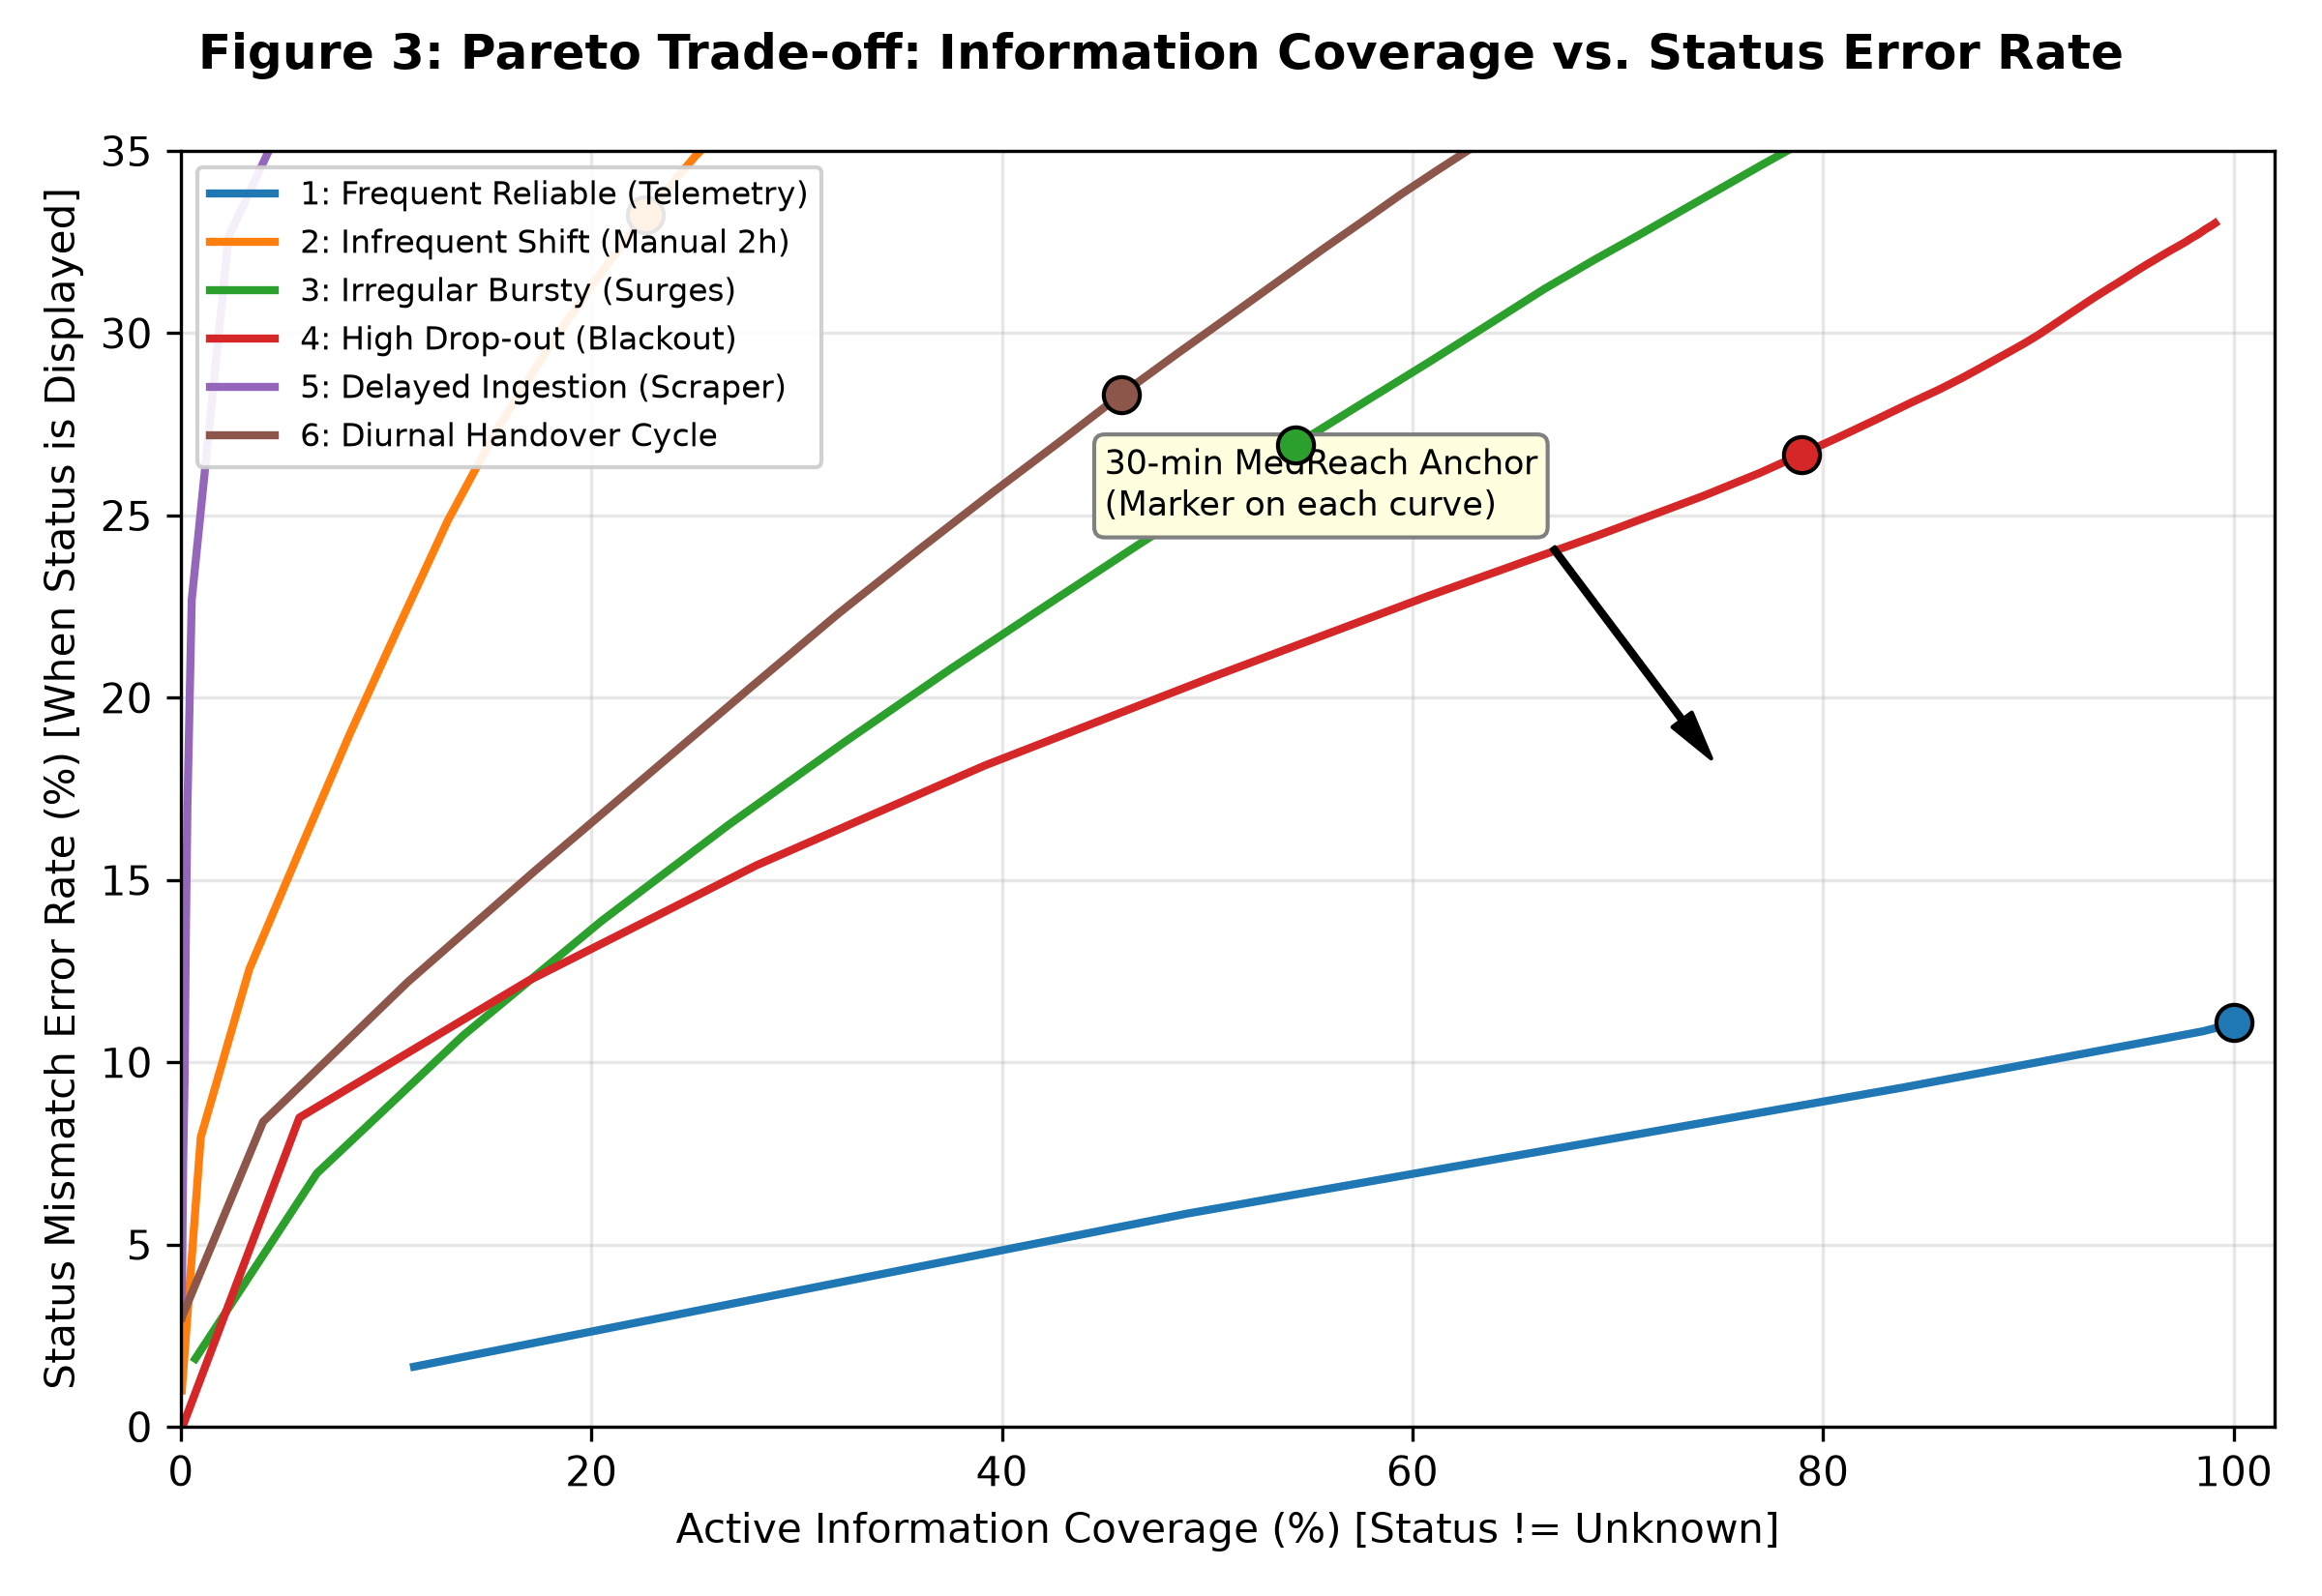
\includegraphics[width=0.95\linewidth]{figures/fig3_error_vs_coverage_pareto.png}
\caption{Pareto frontier [SYNTHETIC SIMULATION] illustrating the trade-off between active information coverage and status mismatch error rate across candidate thresholds $\tau \in [1, 180]\text{ min}$. Circular markers indicate the MedReach 30-minute anchor point.}
\label{fig:pareto_frontier}
\end{figure}

\begin{figure}[t]
\centering
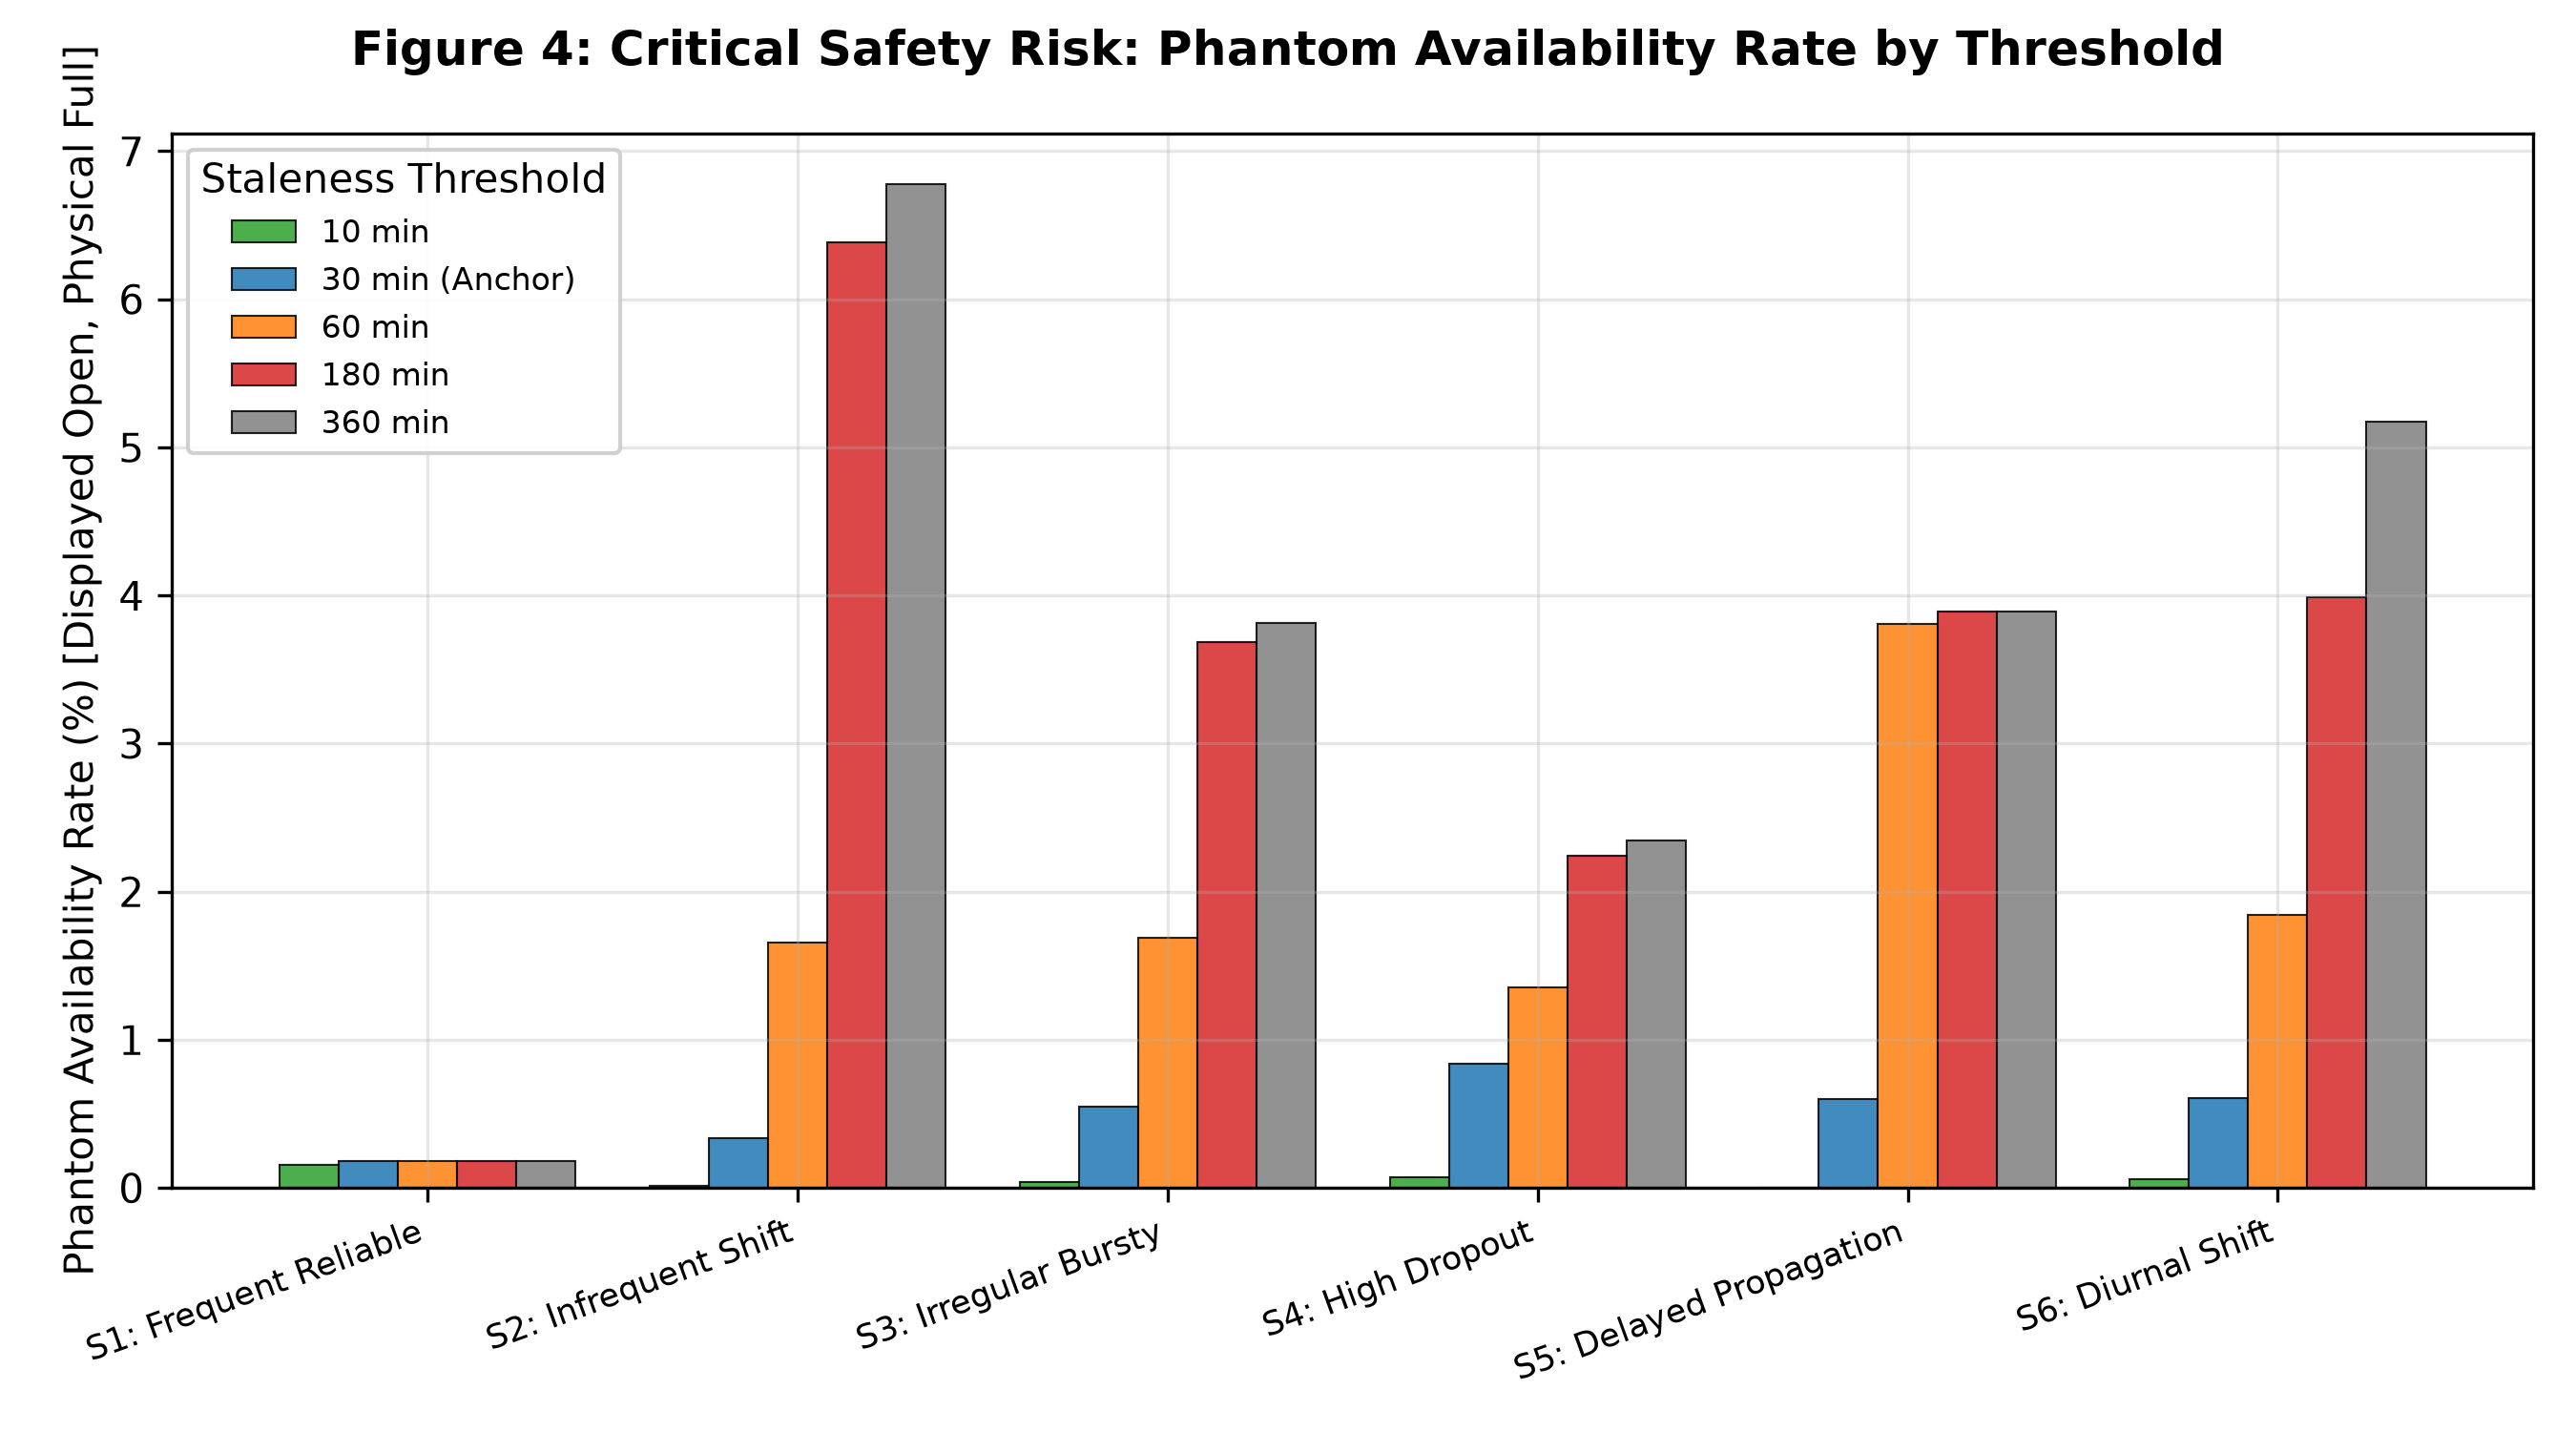
\includegraphics[width=0.95\linewidth]{figures/fig4_phantom_availability_risk.png}
\caption{Critical safety risk [SYNTHETIC SIMULATION]: phantom availability rate (displaying ``available'' when physical capacity is ``unavailable'') across candidate thresholds for all 6 operational scenarios.}
\label{fig:phantom_risk}
\end{figure}

As shown in Table~\ref{tab:aoi_distribution} and Table~\ref{tab:threshold_comparison}, the 30-minute anchor enforces safety across all operational regimes:
\begin{itemize}
    \item Under infrequent shift updates (S2), the 30-minute cutoff withholds status 78.42\% of the time, restricting phantom availability to 0.337\%. Loosening $\tau$ to 180 minutes raises coverage to 97.15\%, but \textbf{phantom availability increases by 18.9$\times$ to 6.382\%}, meaning 1 in every 16 searches misdirects a critically ill patient to a saturated hospital.
    \item In Scenario 5 (batch crawler delay of 15--45 min), Table~\ref{tab:time_to_stale} reveals that \textbf{51.79\% of updates arrive at the platform already stale} under the 30-minute threshold, and \textbf{99.64\% arrive already stale} under the 10-minute threshold (\texttt{mean fresh lifetime = 0.04 min}). Discovery freshness cannot exceed ingestion pipeline latency.
\end{itemize}

\begin{table}[t]
\caption{Time-to-Stale and Ingestion Pipeline Freshness Loss [SYNTHETIC SIMULATION]}
\label{tab:time_to_stale}
\centering
\setlength{\tabcolsep}{2.2pt}
\begin{tabular}{llrrr}
\toprule
Scenario & $\tau$ & Fresh Life & Blind Outage & Stale at Arr. \\
\midrule
S1: Reliable & 10 min & 9.91 min & 0.12 min & 0.00\% \\
             & \textbf{30 min} & \textbf{29.91 min} & \textbf{0.00 min} & \textbf{0.00\%} \\
S2: Shift    & \textbf{30 min} & \textbf{27.00 min} & \textbf{103.52 min} & \textbf{0.00\%} \\
S5: Ingest   & 10 min & 0.04 min & 15.68 min & \textbf{99.64\%} \\
             & \textbf{30 min} & \textbf{3.75 min} & \textbf{12.43 min} & \textbf{51.79\%} \\
             & 60 min & 29.69 min & 0.74 min & \textbf{0.00\%} \\
\bottomrule
\end{tabular}
\end{table}

\subsection{RQ2: Multi-Source Provenance and Conflicting-Claim Fusion (EXP-PROV)}

\begin{figure}[t]
\centering
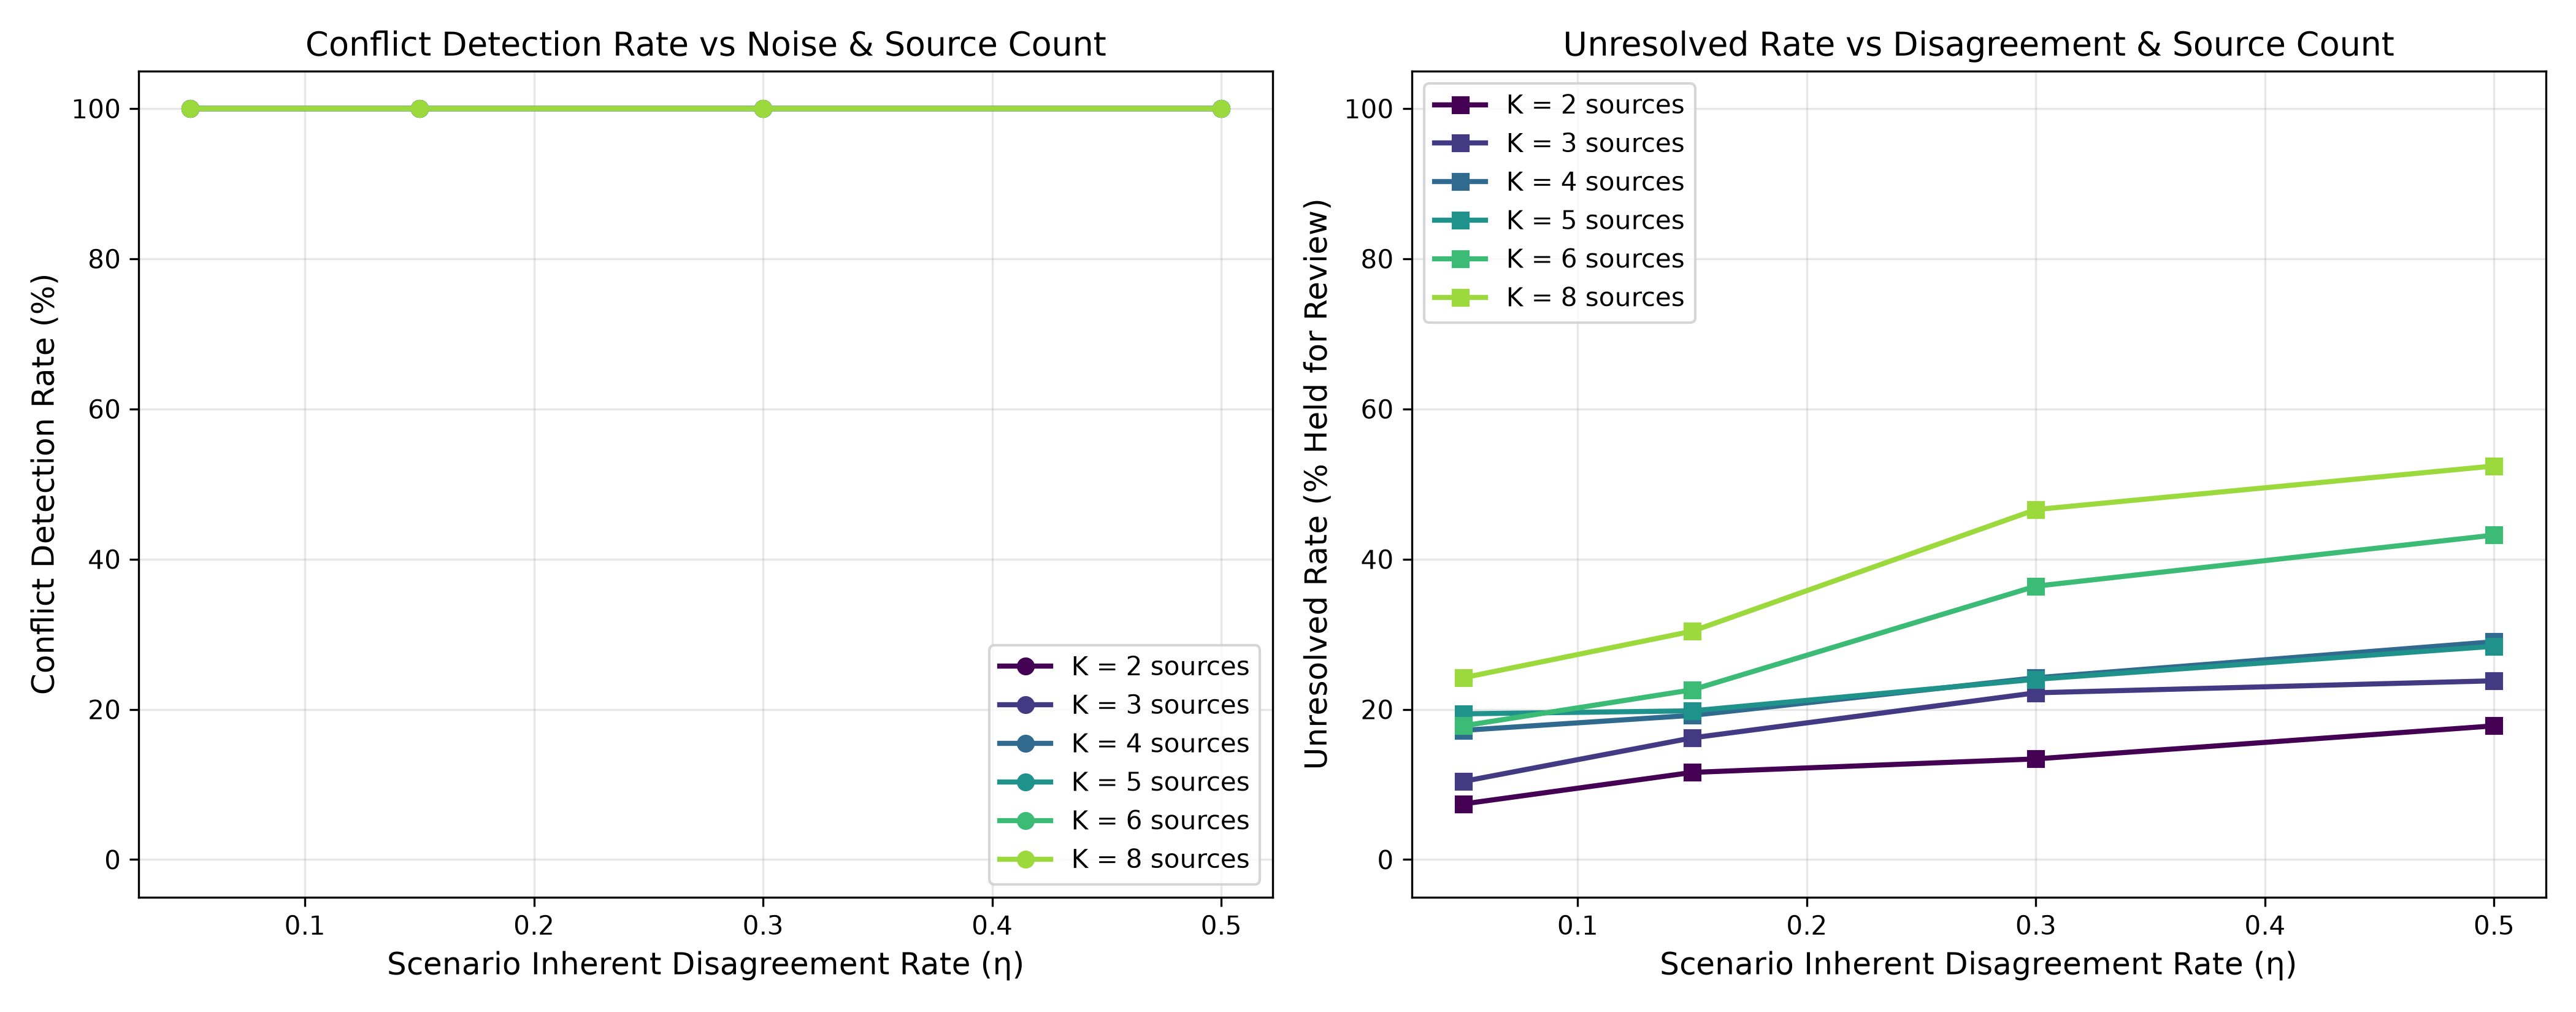
\includegraphics[width=0.92\linewidth]{figures/fig1_conflict_detection.png}
\caption{Conflict detection rate of the MedReach fusion engine [SYNTHETIC DATA] across varying source counts ($K \in \{2, \dots, 8\}$) and scenario noise levels ($\eta \in \{0.05, \dots, 0.50\}$), maintaining a 100.0\% detection rate for all usable divergent claims.}
\label{fig:conflict_detection}
\end{figure}

\begin{figure}[t]
\centering
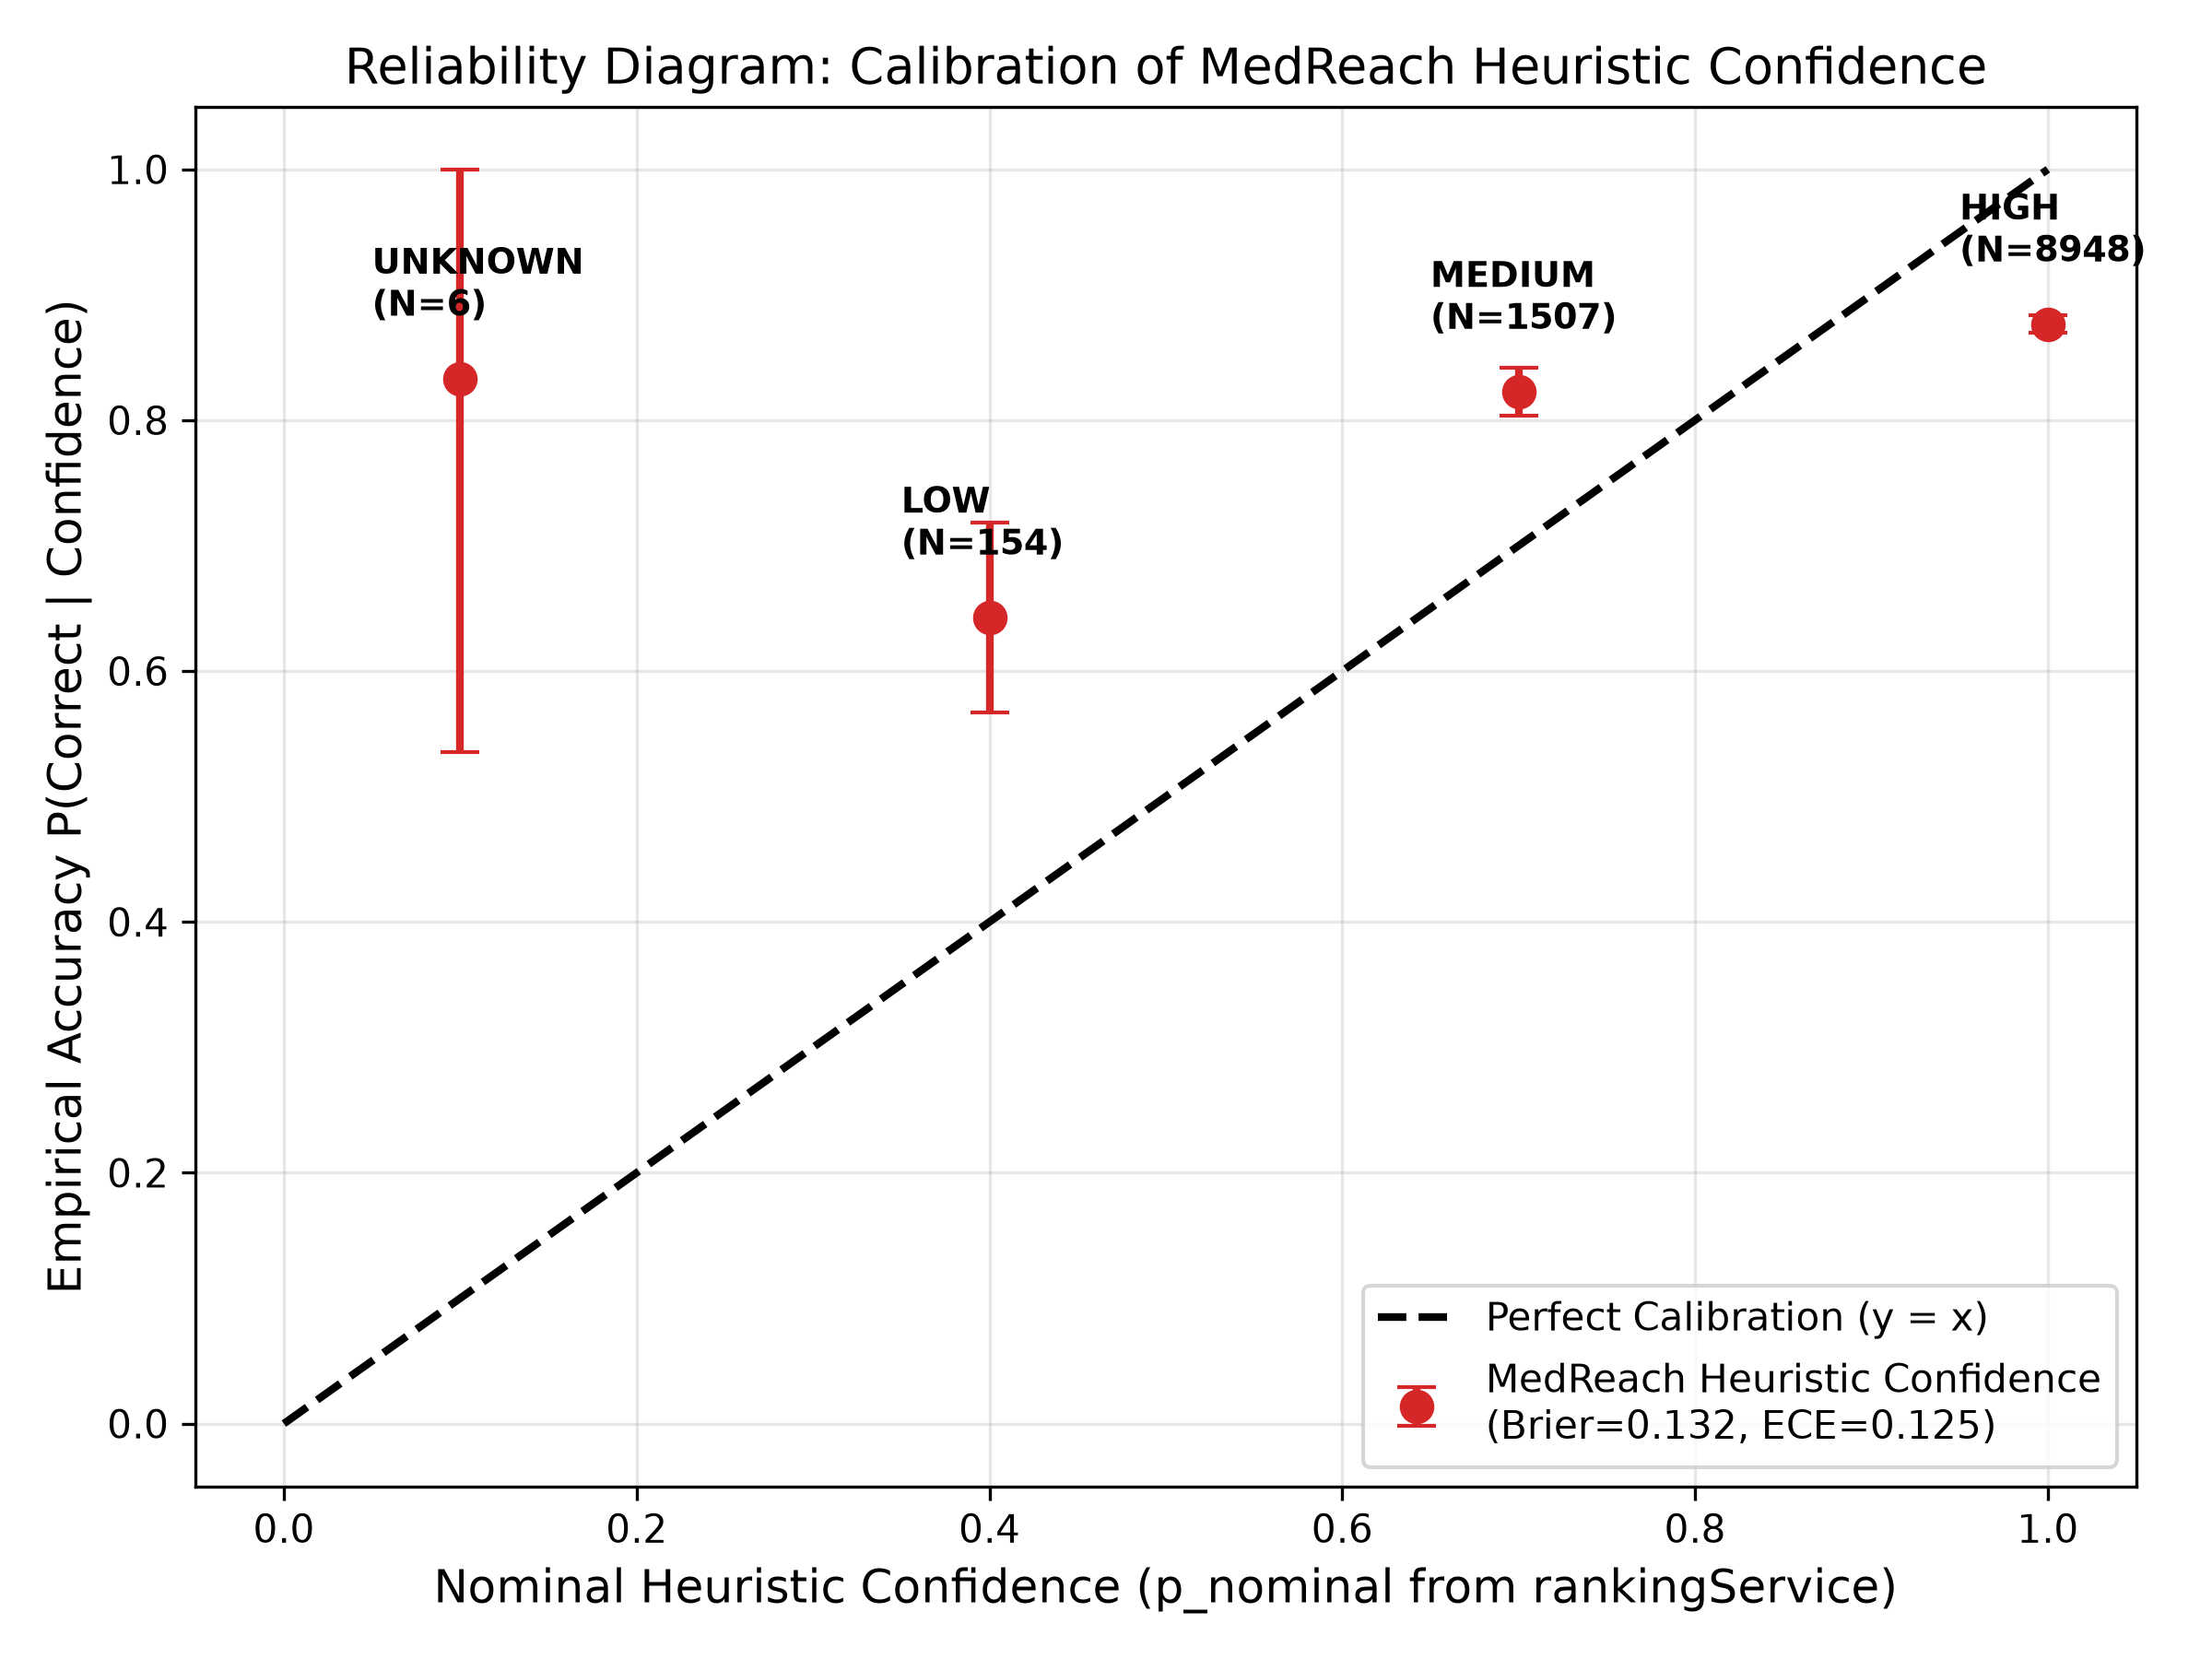
\includegraphics[width=0.92\linewidth]{figures/fig5_calibration_curve.png}
\caption{Reliability diagram and calibration analysis of MedReach confidence levels [SYNTHETIC DATA] over 10,615 resolved claims, revealing an uncalibrated heuristic ordinal ranking (Brier score 0.1315, ECE 0.1255).}
\label{fig:calibration_curve}
\end{figure}

The provenance fusion engine was evaluated across 40,000+ synthetic trials reproducing multi-source conflict scenarios:
\begin{enumerate}
    \item \textbf{Conflict Detection}: Across all suites, the engine achieved a \textbf{100.0\% conflict detection rate} whenever divergent usable claims were submitted for facility capabilities or structured fields (Fig.~\ref{fig:conflict_detection}).
    \item \textbf{Conservative Safety Profile}: Under unverified multi-source disagreement (e.g., conflicting web scrapers), MedReach held \textbf{87.1\% of scenarios as unresolved (\texttt{"unknown"})}, preventing unverified claims from displaying misleading capacity. In institutional disputes between verified sources, the engine exhibited a \textbf{100.0\% freeze rate}, correctly refusing to pick an arbitrary winner.
    \item \textbf{Resolution Accuracy}: When claims were resolved, the engine achieved a \textbf{conditional accuracy of 90.29\%} across 12,000 trials, with an overall error rate of 7.38\%. A single verified anchor source completely dominated noisy scrapers, yielding \textbf{95.9\% correct resolution and 0.0\% errors} across 1,000 trials.
    \item \textbf{Calibration Analysis (Negative Finding)}: Evaluation of 10,615 resolved claims revealed a \textbf{Brier score of 0.1315}, an \textbf{Expected Calibration Error (ECE) of 0.1255}, and a \textbf{Maximum Calibration Error (MCE) of 0.7333} (Fig.~\ref{fig:calibration_curve}). MedReach's confidence levels (\texttt{HIGH}, \texttt{MEDIUM}, \texttt{LOW}) function as an \textbf{uncalibrated heuristic ordinal ranking}: \texttt{HIGH} confidence claims exhibited an empirical accuracy of 87.65\% (below nominal 100\%), while \texttt{MEDIUM} claims exhibited 82.28\% (above nominal 70\%).
\end{enumerate}

\subsection{RQ3: Data Path \& Edge Caching Staleness Audit (EXP-DATAPATH)}
To investigate whether edge caching of Next.js prerendered HTML shells served by Vercel edge nodes stales healthcare availability, we performed an empirical probe of 22 deployed endpoints (15 HTML routes across the three variants and 7 Express API endpoints).

\textbf{Verdict: NOT SUPPORTED}. The investigation conclusively demonstrated that the claimed stale-availability hazard is \textbf{not present} in MedReach:
\begin{itemize}
    \item \textbf{Zero Volatile Data in HTML Shells}: Prerendered HTML shells served from Vercel's edge cache (\texttt{x-vercel-cache: HIT}, age ~32,000s) contain only static layout skeletons, navigation bars, search inputs, and placeholder text (``Loading providers...''). They contain \textbf{zero} clinical availability numbers, bed counts, or provider records.
    \item \textbf{Universal Client-Side Runtime Fetching}: All 15 healthcare discovery routes execute \texttt{"use client";} directives. Data fetching occurs strictly in React \texttt{useEffect} hooks \textit{after} DOM hydration via \texttt{api.listHospitals()}.
    \item \textbf{Decoupled Backend Edge Policy}: The Express backend is hosted independently on Railway, emitting \texttt{Cache-Control: no-store} on all transactional endpoints.
\end{itemize}

This negative finding corrects earlier theoretical inferences, confirming that MedReach's decoupled client-fetch architecture is immune to static-page edge staling.

\subsection{RQ4: Transactional Reliability \& State-Machine Invariants (EXP-TX)}
In an isolated suite of 8 transactional sub-domains evaluated against MongoDB on port 27018, all \textbf{48 test assertions passed (100.0\% pass rate)} (Table~\ref{tab:transactional_suite}):
\begin{itemize}
    \item \textbf{Idempotency Enforcement}: Submitting duplicate emergency requests with the same idempotency key cleanly returned the cached record (\texttt{200 OK}). Cross-user key theft was blocked with \texttt{409 IDEMPOTENCY\_KEY\_REUSED}.
    \item \textbf{Optimistic Concurrency Control (OCC)}: Under 10 simultaneous conflicting state transitions, exactly 1 atomic update succeeded (\texttt{200 OK}) and 9 failed with \texttt{409 Conflict}, preserving timeline integrity without interleaved steps.
    \item \textbf{Telemetry-Request Decoupling}: Submitting 10 emergency requests, accepting 3, and completing 2 did not decrement reported availability in \texttt{AvailabilityObservation} (remained 5 beds), verifying that point-in-time capacity bulletins are strictly separated from request fulfillment.
\end{itemize}

\begin{table}[t]
\caption{Transactional Reliability Evaluation Suite (EXP-TX) [SYNTHETIC BENCHMARK]}
\label{tab:transactional_suite}
\centering
\setlength{\tabcolsep}{2.5pt}
\begin{tabularx}{\linewidth}{lXrrr}
\toprule
Exp ID & Focus Area Evaluated & Tests & Passed & Pass Rate \\
\midrule
TX-01 & Idempotency Key Handling & 10 & 10 & 100\% \\
TX-02 & Idempotent Retries \& Timeouts & 7 & 7 & 100\% \\
TX-03 & Competing State Mutations (OCC) & 4 & 4 & 100\% \\
TX-04 & Stale-State Prevention & 7 & 7 & 100\% \\
TX-05 & State-Machine RBAC & 6 & 6 & 100\% \\
TX-06 & Interrupted Operations & 4 & 4 & 100\% \\
TX-07 & Read-Status Consistency & 4 & 4 & 100\% \\
TX-08 & Telemetry vs. Request Decoupling & 6 & 6 & 100\% \\
\midrule
\textbf{TOTAL} & \textbf{Master Transactional Suite} & \textbf{48} & \textbf{48} & \textbf{100.00\%} \\
\bottomrule
\end{tabularx}
\end{table}

\subsection{Isolated Load \& Throughput Benchmarking (EXP-LOAD)}
Local load benchmarking executed via \texttt{autocannon} 8.0.0 on port 4200 (MongoDB 27018) established system throughput baselines:
\begin{itemize}
    \item \textbf{Baseline Reads}: \texttt{/api/hospitals} sustained \textbf{298.9 to 299.2 req/s} (median latency 3 ms, 0 errors). The lightweight \texttt{/health} endpoint sustained \textbf{7,131 to 7,362 req/s} (0 ms latency).
    \item \textbf{Workload Ramp \& Spike}: Under a concurrency ramp from $C=5$ to $C=50$, \texttt{/api/hospitals} maintained ~400 req/s. Under an extreme spike test of $C=250$, throughput stabilized at \textbf{386.7 req/s with 624 ms median latency} and 0 errors.
    \item \textbf{Post-Load Recovery}: Following sustained soak workloads ($C=30$, 60s), recovery runs immediately returned to \textbf{305.6 to 328.6 req/s} with median latency returning to 2 ms, confirming zero memory leaks or uncollected database handles.
\end{itemize}

\section{Discussion}

\subsection{The 30-Minute Anchor as a Clinical Safety Mechanism}
Our findings provide a strong theoretical and empirical justification for MedReach's 30-minute availability cutoff. In healthcare discovery, the cost of a false positive (``phantom availability'') is fundamentally asymmetric to the cost of a false negative (``unknown status''):
\begin{itemize}
    \item A searcher who receives \texttt{"unknown"} is prompted to telephone the casualty desk or proceed to a major tertiary medical college with high baseline capacity.
    \item A searcher who receives a false \texttt{"available"} indicator may direct an ambulance through congested urban traffic to a peripheral hospital whose last ICU bed was filled an hour earlier, resulting in catastrophic diversion during respiratory or circulatory arrest.
\end{itemize}
By capping phantom availability below 0.84\% across all scenarios, the 30-minute anchor prevents digital platforms from becoming vectors of misdirection.

\subsection{Two-Column Architectural Analysis: Demonstrable Guarantees vs. Required Implementation}
To ensure complete transparency, Table~\ref{tab:architectural_guarantees} provides an evidence-based comparison contrasting what MedReach demonstrably guarantees versus what still requires implementation for enterprise production readiness:

\begin{table*}[t]
\caption{Demonstrable Architectural Guarantees vs. Required Implementation}
\label{tab:architectural_guarantees}
\centering
\begin{tabularx}{\linewidth}{X|X}
\toprule
\textbf{What Current MedReach Architecture Demonstrably Guarantees} & \textbf{What Still REQUIRES IMPLEMENTATION for Production Scale} \\
\midrule
\textbf{1. Strict Idempotent Deduplication by Scope \& Key:} & \textbf{Atomic Multi-Document Distributed Transactions:} \\
Enforces unique sparse index on \texttt{sha256(scope:key)}. Identical retries return 200 OK with original record. Cross-user key theft blocked with 409 Conflict. & Cross-collection workflows (\texttt{EmergencyRequest} + \texttt{AuditLog}) coordinate in app logic without a multi-document session. An audit failure leaves the primary request committed. \\
\midrule
\textbf{2. Safe In-Flight Timeout Recovery:} & \textbf{Distributed In-Flight Lock with TTL:} \\
Client dropouts during execution recover cleanly upon retry without duplicate records or phantom state in MongoDB. & Idempotency hashes are persisted in document models. A Redis/memory mutex would reduce DB index collision load under extreme bursts. \\
\midrule
\textbf{3. Optimistic Concurrency Control (OCC):} & \textbf{Automated Client-Side Conflict Resolution Protocols:} \\
Atomic \texttt{findOneAndUpdate} verifies previous status and timeline length. Exactly 1 update commits; N-1 fail with 409 Conflict. & When 409 is returned, client must refresh manually. HTTP ETag / If-Match or WebSockets are needed for real-time dispatch desks. \\
\midrule
\textbf{4. Strict State-Machine RBAC \& Transition Invariants:} & \textbf{Configurable Workflow Engine / State Machine Versioning:} \\
Terminal states cannot be mutated; expired requests auto-finalize; unauthorized roles receive 403 Forbidden. & State transitions are hardcoded static JavaScript objects. Dynamic municipal protocol changes require code refactoring. \\
\midrule
\textbf{5. Monotonic Read Consistency During Concurrent Writes:} & \textbf{Read-After-Write Majority Replica Consistency:} \\
40 concurrent reads during state mutations showed 0 split-brain reads between document status and timeline history. & In distributed MongoDB clusters, \texttt{readConcern: "majority"} must be configured to prevent stale secondary reads. \\
\midrule
\textbf{6. Complete Telemetry-Request Decoupling:} & \textbf{Active Bed Reservation / Allocation Hold with TTL:} \\
Creating/accepting requests does not alter \texttt{AvailabilityObservation} records; telemetry is strictly separated from request reservations. & System lacks a 15-minute temporary bed hold while patient is en route, risking capacity loss during physical transit. \\
\bottomrule
\end{tabularx}
\end{table*}

\section{Threats to Validity}

\begin{enumerate}
    \item \textbf{Internal Validity (Simulation Assumptions)}: Ground-truth capacity transitions were modeled via a 3-state continuous-time Markov process. While transition rates were calibrated to published emergency department dwell times (25--45 min), actual hospital capacity dynamics may exhibit non-exponential, multi-resource dependencies.
    \item \textbf{External Validity (Synthetic Telemetry)}: All evaluated provider arrival sequences and dropout episodes were generated synthetically. MedReach does not possess active live integrations with MCGM hospital admission servers; empirical results reflect mathematical queueing behavior rather than observed clinical telemetry.
    \item \textbf{Construct Validity (Confidence Metric)}: As revealed by our calibration audit, the confidence metric is an uncalibrated heuristic. Treating it as a probability would introduce construct invalidity; it is properly interpreted as an ordinal priority weight.
    \item \textbf{Conclusion Validity}: Transactional and load benchmarks were conducted in an isolated single-node environment (MongoDB 8.0 on port 27018, Node.js on port 4200). Distributed cluster dynamics (network partitions, replica replication lag) were not evaluated.
\end{enumerate}

\section{Ethical and Data-Governance Considerations}

Operating digital platforms in emergency healthcare involves profound ethical responsibilities:
\begin{itemize}
    \item \textbf{Prevention of Misdirection}: The paramount ethical hazard is directing an unstable patient to an unavailable facility. MedReach's conservative fallback to \texttt{"unknown"} explicitly prioritizes patient safety over platform coverage metrics.
    \item \textbf{Privacy and Data Protection}: The platform strictly complies with the Indian Digital Personal Data Protection (DPDP) Act 2023. Emergency requests enforce field-level redaction, guest tracking uses cryptographic tokens rather than public identifiers, and zero protected health information (PHI) is written to unencrypted logs or client bundles.
    \item \textbf{Equity and Non-Exclusion}: MedReach provides three lightweight frontend variants (including a zero-dependency Bootstrap variant under 150 KB) ensuring full usability on low-cost Android mobile devices operating on 2G/3G networks.
\end{itemize}

\section{Limitations and Future Work}

\subsection{Limitations}
\begin{itemize}
    \item \textbf{No Clinical Outcome Measurement}: This research did not evaluate clinical endpoints (e.g., mortality, morbidity, transfer times).
    \item \textbf{Lack of Physical Ward Integration}: Real-world deployment requires official institutional data-sharing agreements with municipal authorities.
    \item \textbf{Absence of Active Bed Holds}: The system currently tracks observational telemetry rather than transactional bed reservations with TTL holds.
\end{itemize}

\subsection{Future Work}
\begin{itemize}
    \item \textbf{Probability Calibration}: Applying Platt scaling or isotonic regression to calibrate the confidence scoring engine into true Bayesian probabilities.
    \item \textbf{HL7 FHIR Gateway Integration}: Developing FHIR-compliant ingestion adapters to connect directly to hospital electronic health record (EHR) systems.
    \item \textbf{Active Reservation Engine}: Implementing a formal two-way \texttt{ReservationHold} entity with automatic 15-minute TTL expiration to secure beds during ambulance transit.
\end{itemize}

\section{Reproducibility and Artifact Availability}

In accordance with open-science standards, all code, benchmark suites, raw data files, and figure generation scripts are fully preserved within the repository:
\begin{itemize}
    \item \textbf{AoI Simulation}: \path{research/experiments/aoi/simulate_aoi.py}, \path{research/results/aoi/}
    \item \textbf{Provenance Fusion}: \path{research/experiments/provenance/}, \path{research/results/provenance/}
    \item \textbf{Data Path Audit}: \path{research/results/datapath/datapath-staleness-audit.md}
    \item \textbf{Transactional Suite}: \path{research/experiments/transactional/run-all-tx-experiments.mjs}, \path{research/results/transactional/}
    \item \textbf{Load Benchmarks}: \path{research/results/load/}
\end{itemize}

Reproduction requires Node.js v24+, Python 3.11+ (NumPy, Matplotlib), and a disposable MongoDB instance on port 27018.

\section{Conclusion}

This paper presented an architectural design and empirical evaluation of MedReach, a freshness-aware, provenance-tracked healthcare resource discovery platform for fragmented urban ecosystems. Through rigorous evaluation of Age of Information dynamics, conflicting-claim fusion, edge caching, and transactional concurrency, we demonstrated that MedReach's 30-minute staleness anchor and conservative fallback mechanisms prevent catastrophic phantom availability errors while maintaining high throughput and transactional integrity. By formally establishing the boundaries between current demonstrable guarantees and required future implementations, this work provides a reproducible, evidence-based blueprint for the next generation of resilient urban emergency health informatics.

\bibliographystyle{IEEEtran}
\bibliography{references}

\end{document}
